% Modelo adaptado de ../pdf_template/Monografias.v2026.pdf.
% Compilador: LuaLaTeX (Times New Roman e Arial instaladas no sistema).
\documentclass{packages/monografias}
\graphicspath{{figures/}{images/}}
% Identificação consolidada a partir do contexto fornecido pelo autor.
% O título descreve o recorte executado; ver ALINHAMENTO_PROPOSTA.md.
\titulo{Reconstrução virtual de temperaturas a partir de sensores IoT no LASDPC}
\autor[Ferreira]{Gustavo Moura Scarenci de Carvalho Ferreira}
\orientador[Orientador:]{Prof. Dr.}{Júlio Cezar Estrella}
\curso{Engenheiro de Computação}
\disciplina{SSC0670 -- Projeto de Formatura I}
\area{Sensoriamento virtual e análise de dados de sensores IoT}
\local{São Carlos -- SP}


\begin{document}
\imprimircapa
\imprimirfolhaderosto
\pretextual
% Epígrafe, dedicatória e agradecimentos são opcionais.
\begin{resumo}
Este trabalho avalia a reconstrução virtual de temperaturas com dados
históricos de sensores da Internet das Coisas (IoT) no Laboratório de
Sistemas Distribuídos e Programação Concorrente (LASDPC), da Universidade
de São Paulo. Foram utilizados nove sensores do ambiente 1006, de junho
a julho de 2026, com médias de cinco minutos e 12.892 janelas completas.
Compararam-se média aritmética, regressão linear e Random Forest,
com divisão cronológica de 70\% para treinamento e 30\% para teste.
Os erros absolutos médios entre os nove alvos foram, respectivamente,
0,927~°C, 0,257~°C e 0,254~°C, com vantagens distintas por dispositivo.
Na regressão linear com seleção por correlação no treinamento, quatro
entradas apresentaram o menor erro médio entre as quantidades avaliadas,
de 0,238~°C. Na análise espacial com seis sensores, a correlação
apresentou menor erro médio que a proximidade para uma a quatro entradas.
O acréscimo de umidade reduziu pouco o erro médio e apresentou
efeitos distintos por alvo. Os registros de energia foram limitados
a uma auditoria exploratória por sua baixa disponibilidade.
Um mapa das médias representou os pontos observados e a divisória,
com interpolação ilustrativa fora do cluster. Os resultados sustentam
a reconstrução nas condições estudadas, sem assegurar desempenho
equivalente em outros períodos ou ambientes.
\palavraschave{sensoriamento virtual, temperatura, Internet das Coisas,
regressão, séries temporais}
\end{resumo}

\tableofcontents
\clearpage

\textual
\chapter{Introdução}
\label{sec:introducao}

\section{Contextualização e Motivação}
O monitoramento de condições ambientais em espaços internos desempenha um papel importante na caracterização e no acompanhamento das condições de funcionamento desses ambientes. Entre as variáveis frequentemente monitoradas, a temperatura se destaca por sua relação com o conforto térmico, com o funcionamento de equipamentos e com as condições de operação de determinados espaços. Nesse contexto, a utilização de dispositivos conectados à Internet das Coisas (Internet of Things — IoT) permite realizar medições periódicas e armazenar grandes volumes de dados para posterior análise.

Sistemas de monitoramento baseados em sensores distribuídos possibilitam acompanhar a evolução temporal da temperatura em diferentes posições de um ambiente. Entretanto, as medições obtidas por esses dispositivos representam apenas as condições observadas em seus respectivos pontos de instalação. A distribuição espacial da temperatura pode não ser uniforme, especialmente em ambientes que apresentam equipamentos eletrônicos, sistemas de climatização, divisórias e diferentes condições de circulação de ar. Dessa forma, a temperatura registrada em um determinado ponto não necessariamente representa a temperatura de todo o espaço monitorado.

Uma alternativa para ampliar o aproveitamento das informações disponíveis é o emprego de técnicas de sensoriamento virtual, como discutido por \citeonline{brunello2021virtual}. Diferentemente de um sensor físico, que realiza diretamente a medição de uma grandeza, um sensor virtual utiliza informações provenientes de outras fontes para estimar o valor dessa grandeza. No monitoramento térmico, essa abordagem permite investigar a possibilidade de estimar a temperatura em uma determinada posição a partir das medições realizadas por sensores instalados em outras posições.

A viabilidade dessa abordagem depende, entre outros fatores, das relações existentes entre as séries temporais dos sensores, da distribuição espacial dos dispositivos e do método utilizado para realizar as estimativas. Sensores próximos podem apresentar comportamentos semelhantes, mas essa relação não é necessariamente determinada apenas pela distância física. Características específicas do ambiente também podem influenciar as medições e, consequentemente, a precisão das estimativas.

Nesse cenário, métodos estatísticos e de aprendizado de máquina podem ser empregados para identificar relações entre as temperaturas registradas por diferentes dispositivos. Modelos como regressão linear e Random Forest permitem construir estimativas a partir de observações históricas, oferecendo alternativas a estratégias mais simples, como o cálculo da média das temperaturas dos sensores disponíveis.

O presente trabalho investiga a reconstrução virtual de medições de temperatura utilizando dados históricos de sensores IoT instalados em ambientes internos de laboratório. O estudo considera uma infraestrutura de monitoramento já existente, sem alterações no posicionamento físico dos dispositivos. Dessa forma, a investigação concentra-se no aproveitamento dos dados disponíveis e na avaliação de diferentes estratégias de estimativa.

Para possibilitar a avaliação quantitativa dos métodos, adota-se uma abordagem na qual as medições de um sensor físico são utilizadas como referência, enquanto as medições dos demais sensores servem como entradas para os modelos. Assim, é possível comparar as temperaturas estimadas com os valores efetivamente registrados e quantificar os erros de reconstrução.

Além da comparação entre diferentes modelos, o trabalho busca investigar como a quantidade de sensores utilizados e os critérios empregados para sua seleção influenciam a qualidade das estimativas. Para isso, são consideradas tanto as relações estatísticas entre as séries temporais quanto as informações aproximadas sobre a localização física dos dispositivos.

\section{Delimitação e Evolução do Escopo}
\label{sec:evolucao_escopo}

A proposta inicial, intitulada \textit{Enriquecimento de Dados de Sensores
IoT para Aprendizado de Máquina focado em Conforto Térmico no LASDPC},
previa estruturar os históricos e associá-los à localização física,
aos estados da climatização e a outras informações para apoiar modelos
de estimativa térmica e inferência de conforto. O presente documento
explicita o recorte efetivamente executado: a reconstrução de temperaturas
registradas por sensores físicos, com referência observada para avaliação.

A preparação dos dados resultou em matrizes temporais sincronizadas.
O enriquecimento foi operacionalizado pela associação dos identificadores
ao cadastro e às coordenadas, e pela integração da umidade às entradas
dos modelos. A regressão linear e a Random Forest constituem as abordagens
de aprendizado supervisionado avaliadas. As coordenadas apoiam a seleção
por proximidade e a representação espacial; não foram adicionadas como
variáveis explicativas dos modelos individuais de cada alvo.

O conforto térmico permanece como motivação e possibilidade de aplicação.
Não foram coletadas todas as variáveis necessárias a uma avaliação de
conforto, nem respostas dos ocupantes que permitissem validá-la. Também
não foram integradas informações meteorológicas externas ou estados
confirmados dos aparelhos de climatização. Os registros de energia foram
limitados a uma auditoria, devido à curta disponibilidade e à unidade
não confirmada do campo consultado.

Assim, a contribuição apresentada está na estruturação, no enriquecimento
e na avaliação dos dados para sensoriamento virtual. O mapa permite
visualizar diferenças entre temperaturas médias em posições conhecidas,
mas não representa a validação de um gradiente térmico contínuo ou de
condições de conforto. A inferência de conforto e o controle automatizado,
previstos como aplicações na proposta inicial, dependem de uma etapa
adicional de instrumentação e definição do protocolo de avaliação.

\section{Objetivos}
No recorte delimitado, o objetivo geral é avaliar a reconstrução virtual
de temperaturas a partir de dados históricos de sensores IoT,
estruturados e enriquecidos com cadastro espacial e umidade,
utilizando medições físicas como referência experimental.

Como objetivos específicos, estabelecem-se:
\begin{itemize}
    \item caracterizar os dados históricos e a disponibilidade das medições;
    \item organizar os sensores por identificadores cadastrais e posições relativas;
    \item preparar e sincronizar as séries em uma grade temporal comum;
    \item comparar média aritmética, regressão linear e Random Forest;
    \item investigar o efeito da quantidade de sensores de entrada;
    \item comparar seleção por correlação e proximidade no subconjunto com coordenadas;
    \item avaliar a umidade dos sensores de entrada como informação complementar
    à reconstrução de temperatura;
    \item interpretar os erros por sensor e representar espacialmente as temperaturas médias.
\end{itemize}

\section{Organização do Trabalho}
Este trabalho está organizado em quatro capítulos. O
Capítulo~\ref{sec:revisao} apresenta os conceitos de sensoriamento virtual,
séries temporais e métodos de estimativa, além dos trabalhos relacionados.
O Capítulo~\ref{sec:desenvolvimento} descreve a infraestrutura, os dados,
o pré-processamento e o protocolo de avaliação, e apresenta os resultados
e suas limitações. O Capítulo~\ref{sec:conclusao} reúne as conclusões e as
possibilidades de continuidade da pesquisa.

\chapter{Revisão Bibliográfica}
\label{sec:revisao}

\section{Considerações Iniciais}

A reconstrução de temperaturas a partir de redes de sensores envolve
relações entre as medições, disponibilidade dos registros e escolha das
entradas. Este capítulo apresenta os conceitos de monitoramento IoT,
séries temporais e sensoriamento virtual, seguidos dos métodos de
estimativa e das pesquisas que fundamentam a avaliação experimental.

\section{Conceitos e Técnicas Relevantes}
\label{sec:conceitos}

\subsection{Monitoramento Ambiental e Internet das Coisas}
\label{subsec:iot}

A Internet das Coisas (\textit{Internet of Things} -- IoT) integra
dispositivos de aquisição, comunicação e serviços que disponibilizam
medições para acompanhamento e análise. Em aplicações ambientais,
sensores distribuídos registram grandezas como temperatura e umidade,
produzindo séries associadas a diferentes posições físicas.

\citeonline{marques2026testbed} descrevem uma infraestrutura de laboratório
com dispositivos ESP32, comunicação multiprotocolo e armazenamento de
séries temporais. A disponibilidade de históricos dessa infraestrutura
permite investigar o aproveitamento conjunto das medições, além do
monitoramento direto de cada dispositivo. Contudo, a presença de um
registro no banco não assegura continuidade, sincronização ou
representatividade de todas as posições do ambiente.

\subsection{Séries Temporais e Pré-processamento de Dados}
\label{subsec:series_temporais}

Uma série temporal reúne observações associadas a instantes ou
intervalos de tempo. Sensores podem registrar valores em instantes
diferentes e apresentar lacunas, mesmo quando possuem frequências
nominais semelhantes. A análise conjunta exige verificar identificadores,
convenções temporais, duplicatas, valores inválidos e disponibilidade
simultânea.

Uma estratégia de sincronização é agregar as medições em intervalos
regulares. Para o sensor $s$ e a janela $t$, a média é
\begin{equation}
    \overline{T}_{s,t}=\frac{1}{n_{s,t}}
    \sum_{j=1}^{n_{s,t}}T_{s,t,j},
    \label{eq:media_temporal}
\end{equation}
em que $n_{s,t}>0$ é a quantidade de medições disponíveis e $T_{s,t,j}$
a $j$-ésima temperatura da janela. Intervalos maiores reduzem a resolução
temporal e podem facilitar a coincidência dos registros, enquanto
intervalos menores preservam variações mais rápidas.

Valores ausentes podem ser preservados, excluídos ou imputados, conforme
o objetivo e as características dos dados. \citeonline{alsalehy2025timeseries}
discutem a importância de considerar a estrutura temporal na detecção
de anomalias e no preenchimento de lacunas ambientais. Qualquer regra
adotada deve ser documentada para permitir interpretar suas consequências
sobre o conjunto efetivamente avaliado.

\subsection{Aprendizado de Máquina e Enriquecimento dos Dados}
\label{subsec:ia_enriquecimento}

O aprendizado de máquina é a abordagem de inteligência artificial (IA)
empregada neste estudo. No aprendizado supervisionado, observações
históricas relacionam variáveis de entrada a uma resposta conhecida,
permitindo ajustar um modelo e avaliar suas estimativas em outras
observações. A Scikit-learn disponibiliza implementações para esse
procedimento \cite{pedregosa2011scikit}; entre os métodos estudados,
a Random Forest combina árvores de decisão \cite{breiman2001random}.

O enriquecimento amplia as informações associadas aos registros.
No contexto deste trabalho, compreende vincular as medições a metadados
dos dispositivos e às posições físicas, além de combinar temperatura
e umidade em uma mesma janela temporal. As informações espaciais podem
orientar a seleção de entradas, enquanto a inclusão de outra grandeza
ambiental permite investigar sua contribuição preditiva. O benefício
precisa ser demonstrado na avaliação, pois aumentar as informações
não assegura menor erro.

A integração de grandezas ambientais e registros de energia também
é explorada por \citeonline{tavoni2026digitaltwin}, que utilizam essas
informações na previsão de consumo em uma arquitetura de gêmeo digital.
Essa relação oferece contexto para o enriquecimento investigado aqui,
embora a variável de resposta e o sistema desenvolvido sejam distintos.

\subsection{Sensoriamento Virtual de Temperatura}
\label{subsec:sensoriamento_virtual}

Um sensor virtual utiliza informações disponíveis para estimar uma
grandeza que poderia ser medida por um sensor físico. Na reconstrução
de temperaturas, o problema pode ser representado por
\begin{equation}
    \widehat{T}_p(t)=f\bigl(T_1(t),\ldots,T_k(t)\bigr),
    \label{eq:sensoriamento_virtual}
\end{equation}
em que $p$ é o alvo, $k$ é a quantidade de entradas e $f$ é o método
de estimativa. As medições do próprio alvo não podem integrar essas
entradas durante a reconstrução; seu histórico pode fornecer a resposta
para treinamento supervisionado.

\citeonline{brunello2021virtual} investigam essa abordagem em um escritório
com sensores distribuídos irregularmente, combinando seleção de entradas
e avaliação de preditores. A distância física e a correlação entre
séries são critérios distintos: o primeiro utiliza coordenadas, enquanto
o segundo expressa associação entre observações. Mais entradas podem
adicionar informação ou redundância, tornando necessário avaliar seu
efeito em dados separados do ajuste e da seleção.

\subsection{Métodos de Estimativa e Avaliação}
\label{subsec:metodos_estimativa}

A média aritmética constitui uma referência sem treinamento:
\begin{equation}
    \widehat{T}_p(t)=\frac{1}{k}\sum_{i=1}^{k}T_i(t).
    \label{eq:media_sensores}
\end{equation}
Ela atribui pesos iguais às entradas e não ajusta diferenças sistemáticas
entre o nível térmico dos sensores e o do alvo.

A interpolação pelo inverso da distância (\textit{Inverse Distance
Weighting} -- IDW) atribui maior peso a observações próximas:
\begin{equation}
    \widehat{T}_p(t)=
    \frac{\sum_{i=1}^{k}T_i(t)d_{ip}^{-q}}
         {\sum_{i=1}^{k}d_{ip}^{-q}},
    \label{eq:idw}
\end{equation}
em que $d_{ip}>0$ é a distância ao ponto estimado e $q>0$ controla
o decaimento dos pesos. Na coincidência espacial com um sensor,
atribui-se seu valor diretamente. \citeonline{jedermann2011interpolation}
comparam IDW e Kriging na reconstrução de perfis de temperatura.
A interpolação fornece valores entre pontos observados, mas sua
representação gráfica não substitui a validação contra medições.

A regressão linear estima o alvo por uma combinação ajustada das entradas:
\begin{equation}
    \widehat{T}_p(t)=\beta_0+\sum_{i=1}^{k}\beta_iT_i(t),
    \label{eq:regressao_linear}
\end{equation}
em que $\beta_0$ é o intercepto e $\beta_i$ são os coeficientes estimados
no treinamento. A Random Forest, apresentada por
\citeonline{breiman2001random}, combina árvores de decisão; em regressão,
as estimativas das árvores são agregadas. Essa estrutura permite
representar relações não lineares, mas não assegura menor erro que
uma alternativa linear em qualquer conjunto de dados.

A comparação utiliza o erro absoluto médio (\textit{Mean Absolute
Error} -- MAE) e a raiz do erro quadrático médio (\textit{Root Mean
Squared Error} -- RMSE):
\begin{equation}
    \mathrm{MAE}=\frac{1}{n}\sum_{j=1}^{n}|T_j-\widehat{T}_j|,
    \label{eq:mae}
\end{equation}
\begin{equation}
    \mathrm{RMSE}=\sqrt{\frac{1}{n}
    \sum_{j=1}^{n}(T_j-\widehat{T}_j)^2}.
    \label{eq:rmse}
\end{equation}
As duas métricas possuem a unidade da temperatura, mas o RMSE penaliza
mais os erros elevados. $T_j$ é o valor observado, $\widehat{T}_j$ é a
estimativa e $n$ é o número de observações. Sua interpretação exige
informar a divisão temporal, os alvos e as amostras utilizados.

\subsection{Relação com o Conforto Térmico}
\label{subsec:conforto_termico}

Temperatura e umidade são relevantes à caracterização ambiental,
mas a interpretação do conforto envolve outras condições. A apresentação
institucional da ASHRAE Standard 55 relaciona fatores ambientais
--- temperatura, radiação térmica, umidade e velocidade do ar ---
e pessoais, como atividade e vestimenta \cite{ashrae55overview}.
Assim, uma temperatura reconstruída com baixo erro não permite,
isoladamente, classificar a satisfação térmica dos ocupantes.

O presente conjunto não inclui caracterização da radiação térmica,
da velocidade do ar, da atividade ou da vestimenta, nem votos de
sensação térmica. Esses fatores não foram substituídos por valores
arbitrários para produzir um índice. A reconstrução e a representação
espacial são tratadas como recursos analíticos que poderiam apoiar
uma avaliação de conforto futura, mediante protocolo e dados adequados.

\section{Trabalhos Relacionados}
\label{sec:trabalhos_relacionados}

\citeonline{marques2026testbed} apresentam uma infraestrutura IoT com
ESP32, MQTT, CoAP, atualização remota de firmware e observabilidade.
Os autores relatam redução de 55,7\% no consumo mensal de energia em
seu cenário de controle de climatização, mantendo condições de conforto.
Essa evidência caracteriza a aplicação da infraestrutura estudada
pelos autores; o presente trabalho utiliza históricos de temperatura
e não reproduz o experimento energético.

\citeonline{tavoni2026digitaltwin} apresentam uma arquitetura modular
de gêmeo digital para otimização energética em um laboratório da USP.
A solução integra sensores de temperatura e umidade DHT22, sensores
de corrente SCT-013, comunicação MQTT, Eclipse Ditto e uma interface
em Unity. O componente preditivo utiliza XGBoost para estimar consumo
em kWh, com valores anteriores de energia, temperatura e umidade,
validação por \textit{TimeSeriesSplit} e parada antecipada no treinamento.

O artigo descreve cenários de simulação com diferentes configurações
de operação e reconhece limitações relacionadas ao período experimental
e à generalização. Sua contribuição para este TCC está na integração
de dados heterogêneos e no uso de aprendizado de máquina para apoiar
análises da climatização. Neste trabalho, a resposta é a temperatura
de um sensor e a avaliação usa uma divisão temporal fixa; não foram
implementados gêmeo digital, XGBoost, simulação de consumo ou atuação.
O SCT-013 descrito pelos autores também difere do modelo ACS712
identificado na extração aqui analisada. Portanto, a unidade kWh
reportada naquele estudo não confirma a unidade do campo
\texttt{energy} deste conjunto.

\citeonline{brunello2021virtual} constituem a referência mais próxima
do problema investigado. Os autores analisam métricas de distância
espaciais e estatísticas, desenvolvem uma combinação por programação
genética e selecionam subconjuntos de sensores para estimar temperaturas
em um escritório. Avaliam diferentes estratégias de predição e a
confiabilidade das saídas. O presente estudo adota uma comparação mais
restrita, com métodos simples e duas regras de seleção, aplicada aos
dispositivos e históricos disponíveis no LASDPC.

\citeonline{yuan2025optimization} investigam reconstrução de campos
térmicos em regimes estacionários e transientes, com cenários numéricos
de condução de calor. Comparam configurações esparsas de sensores e
métodos baseados em decomposição ortogonal própria (\textit{Proper
Orthogonal Decomposition} -- POD), incluindo Gappy POD e Gappy C-POD.
O estudo fundamenta a relevância da configuração das medições. Entretanto,
a otimização de posições em cenários numéricos difere da condição deste
TCC, que utiliza sensores reais previamente instalados.

\citeonline{jedermann2011interpolation} aplicam interpolação espacial
a dados de armazenamento e transporte de alimentos, comparando Kriging
com ponderação pelo inverso da distância. Nos conjuntos avaliados pelos
autores, o erro de Kriging foi aproximadamente 20\% menor que o da
referência IDW. O trabalho sustenta a discussão de relações espaciais,
mas não transfere esse resultado diretamente ao ambiente do LASDPC.
Neste TCC, a IDW é usada apenas para ilustrar as médias espaciais.

\citeonline{alsalehy2025timeseries} avaliam identificação de anomalias e
imputação em séries de gases e variáveis meteorológicas, combinando
métodos estatísticos e algoritmos de detecção, além de interpolação
linear, PCHIP e Akima. Sua relação com o presente estudo é a atenção
à continuidade e à qualidade das séries. A decisão experimental aqui
adotada foi selecionar janelas completas, sem reproduzir as técnicas
de imputação desse artigo.

Por fim, \citeonline{cho2022preprocessing} investigam combinações de
tratamento de valores ausentes e desbalanceamento para classificação
industrial. Embora a aplicação seja distinta da reconstrução de
temperaturas, o artigo reforça que a preparação dos dados integra
o procedimento de avaliação e deve ser descrita com precisão.

\section{Considerações Finais}
\label{sec:consideracoes_finais_revisao}

Os trabalhos sobre infraestrutura e gêmeos digitais contextualizam
a integração das medições e suas aplicações na climatização.
A literatura relaciona o sensoriamento virtual à seleção de entradas,
aos métodos de estimativa e à qualidade das medições. Este trabalho
reúne essas perspectivas em uma avaliação delimitada de dados reais,
sem propor um novo algoritmo ou otimizar a posição física dos sensores.
O capítulo seguinte descreve a infraestrutura, os dados e o protocolo,
e apresenta os resultados nas condições efetivamente disponíveis.

\chapter{Desenvolvimento do Trabalho}
\label{sec:desenvolvimento}

\section{Considerações Iniciais}
\label{sec:desenvolvimento_iniciais}

Este capítulo descreve a infraestrutura e o recorte experimental,
a preparação das séries e a avaliação da reconstrução de temperaturas.
Apresenta também os resultados por método e sensor-alvo, a influência
da quantidade de entradas e a análise espacial complementar.

\section{Descrição do Problema e do Ambiente}
\label{sec:descricao_projeto}

\subsection{Problema de reconstrução}
\label{subsec:contextualizacao_problema}
\label{subsec:proposta_reconstrucao}

O problema consiste em estimar a temperatura agregada de um sensor
físico a partir das medições dos demais dispositivos do mesmo ambiente.
A referência física permite quantificar o erro, enquanto o histórico
do alvo fornece a resposta para ajustar os modelos supervisionados.
Durante a estimativa, o valor do alvo não participa das entradas.
A investigação utiliza uma infraestrutura preexistente, sem alterar
o posicionamento dos sensores ou propor novos algoritmos.

\subsection{Ambiente experimental e cadastro}
\label{subsec:ambiente_experimental}

O trabalho utiliza a infraestrutura do Laboratório de Sistemas
Distribuídos e Programação Concorrente (LASDPC), do Instituto de
Ciências Matemáticas e de Computação (ICMC), da Universidade de São
Paulo (USP). O experimento principal considera os registros associados
ao identificador \texttt{1006} no QuestDB.

O cadastro da plataforma e a planta física descrevem aspectos distintos.
As categorias 1006, Cluster e Reunião identificam grupos de dispositivos
no inventário consultado; por si só, esses nomes não definem paredes
ou espaços termicamente isolados. Na planta fornecida pelo autor,
o espaço do cluster é separado da região dos demais sensores por
uma divisória, com abertura à direita. A interpretação espacial considera
essa configuração, e não somente o nome atribuído a cada dispositivo.

As coordenadas são relativas e aproximadas. Foram confirmadas posições
para 14 dispositivos, dos quais seis pertencem ao conjunto principal
de nove sensores. A seleção por distância utiliza apenas esse subconjunto;
os outros três sensores não receberam coordenadas por aproximação.
O mapa da Seção~\ref{subsec:mapa_termico} apresenta os pontos observados,
a divisória e o domínio da interpolação ilustrativa.

\subsection{Infraestrutura de monitoramento e armazenamento}
\label{subsec:infraestrutura_monitoramento}

A infraestrutura está relacionada à plataforma apresentada por
\citeonline{marques2026testbed}, com dispositivos baseados em ESP32,
comunicação e armazenamento de séries temporais. Na exploração do
QuestDB, os dispositivos do conjunto principal foram associados ao
modelo DHT22. A resposta principal é a temperatura; uma análise complementar inclui
umidade como entrada e uma auditoria caracteriza o campo de energia.
Não foi realizado controle de climatização.

No QuestDB, as tabelas identificadas foram
\texttt{sensor\_temperature}, \texttt{sensor\_humidity} e
\texttt{sensor\_energy}. A primeira contém o instante
\texttt{measured\_in}, o identificador \texttt{sensor\_id}, o modelo,
o ambiente e a temperatura. As consultas SQL foram realizadas em
Python, por interface HTTP, e as extrações preservadas localmente.
A API Smartlab foi explorada separadamente para consultar o cadastro
e outros dispositivos. As diferenças de disponibilidade entre as
extrações são discutidas na Seção~\ref{subsec:disponibilidade_fontes}.

\section{Descrição das Atividades Realizadas}
\label{sec:metodologia}

A metodologia foi organizada em etapas de aquisição, preparação e análise dos dados, seguidas pela execução de experimentos de reconstrução virtual de temperaturas. A Figura~\ref{fig:fluxograma_metodologia}
apresenta uma visão geral desse procedimento, destacando o processamento comum das séries temporais e as diferentes configurações experimentais avaliadas. Os experimentos complementares investigam a influência da quantidade e da seleção de sensores de referência, bem como a contribuição da umidade relativa para as estimativas.

\begin{figure}[p]
\centering
\begin{tikzpicture}[
  font=\small,
  >={Latex[length=2mm]},
  node distance=0.55cm,
  etapa/.style={draw=black!65,rounded corners=2pt,fill=blue!6,
    align=center,text width=10.1cm,minimum height=1.00cm,inner sep=5pt},
  ensaio/.style={draw=black!65,rounded corners=2pt,fill=green!7,
    align=center,text width=4.55cm,minimum height=1.75cm,inner sep=5pt},
  saida/.style={draw=black!65,rounded corners=2pt,fill=orange!10,
    align=center,text width=10.1cm,minimum height=1.00cm,inner sep=5pt},
  auxiliar/.style={draw=black!55,dashed,rounded corners=2pt,fill=gray!7,
    align=center,text width=10.1cm,minimum height=0.95cm,inner sep=5pt},
  fluxo/.style={-{Latex[length=2mm]},thick,draw=black!70}
]
\node[etapa] (fonte) {\textbf{Aquisição dos dados}\\QuestDB: ambiente 1006, nove sensores de temperatura};
\node[etapa,below=of fonte] (preparo) {\textbf{Pré-processamento}\\Agregação em 5 minutos e sincronização temporal};
\node[etapa,below=of preparo] (matriz) {\textbf{Matriz experimental}\\12.892 janelas completas de temperatura};
\node[etapa,below=of matriz] (divisao) {\textbf{Divisão cronológica}\\9.024 janelas de treinamento (70\%) e 3.868 de teste (30\%)};
\draw[fluxo] (fonte) -- (preparo);
\draw[fluxo] (preparo) -- (matriz);
\draw[fluxo] (matriz) -- (divisao);

\node[ensaio,below=1.35cm of divisao.south west,anchor=north west,xshift=0.02cm] (exp1) {\textbf{Comparação dos métodos}\\Média aritmética\\Regressão linear e Random Forest\\9 sensores};
\node[ensaio,right=0.65cm of exp1] (exp2) {\textbf{Quantidade de entradas}\\Regressão linear\\Correlação; $k\in\{1,2,3,4,6,8\}$\\9 sensores};
\node[ensaio,below=0.55cm of exp1] (exp3) {\textbf{Seleção espacial}\\Correlação versus\\proximidade\\6 sensores com coordenadas};
\node[ensaio,right=0.65cm of exp3] (exp4) {\textbf{Inclusão de umidade}\\Regressão linear\\Temperaturas versus\\temperaturas + umidades};
\begin{scope}[on background layer]
  \node[draw=black!45,dashed,rounded corners=3pt,fill=gray!3,
    fit=(exp1)(exp2)(exp3)(exp4),inner xsep=0.25cm,
    inner ysep=0.55cm] (grupo) {};
\end{scope}
\node[fill=white,inner sep=2pt,font=\bfseries\small] at ([xshift=-3.05cm]grupo.north) {Experimentos de reconstrução};
\draw[fluxo] (divisao.south) -- (grupo.north);

\node[saida,below=0.70cm of grupo.south] (avaliacao) {\textbf{Avaliação das reconstruções}\\Comparação com os valores observados\\MAE, RMSE e $R^2$};
\node[saida,below=of avaliacao] (analise) {\textbf{Análise e interpretação}\\Comparação por método, sensor-alvo e configuração};
\draw[fluxo] (grupo.south) -- (avaliacao.north);
\draw[fluxo] (avaliacao) -- (analise);

\node[auxiliar,below=0.5cm of analise] (energia) {\textbf{Auditoria independente dos registros de energia}\\Caracterização da disponibilidade; sem entrada nos modelos};
\end{tikzpicture}
\vspace{10pt}
\caption{Visão geral da preparação dos dados, dos experimentos de reconstrução e da avaliação. A análise espacial considera seis sensores com coordenadas conhecidas, e o experimento com umidade utiliza amostras pareadas. A auditoria de energia é independente dos modelos de reconstrução.}
\label{fig:fluxograma_metodologia}
\fautor
\end{figure}

\subsection{Operacionalização do Enriquecimento}
\label{subsec:operacionalizacao_enriquecimento}

A base foi organizada em três níveis. Primeiro, as consultas e a grade
temporal estruturaram as observações para análise conjunta. Em seguida,
os identificadores foram associados ao cadastro e às coordenadas
confirmadas, permitindo comparar critérios de seleção e representar
os sensores. Por fim, a umidade foi alinhada às temperaturas e incluída
nas entradas da regressão linear. Essas etapas são rastreáveis nos
notebooks e nas tabelas exportadas.

% O aprendizado supervisionado utiliza a temperatura do alvo como resposta histórica e as medições dos demais dispositivos como entradas. O experimento com umidade compara oito temperaturas com oito temperaturas e oito umidades, em amostras pareadas. Já as coordenadas são utilizadas no ordenamento por proximidade e no mapa, sem integrar a matriz de variáveis explicativas dos modelos individuais. Dessa forma, o uso espacial e a inclusão de outra grandeza ambiental são avaliados em experimentos complementares, e não como uma única configuração.

O aprendizado supervisionado utiliza a temperatura do sensor-alvo como resposta histórica e as medições dos demais dispositivos como variáveis de entrada. Para avaliar a contribuição da umidade relativa, foram comparadas duas configurações de regressão linear: a primeira utiliza as temperaturas dos oito sensores de referência, enquanto a segunda incorpora também suas respectivas medições de umidade, totalizando 16 variáveis explicativas. Ambas foram avaliadas sobre os mesmos registros temporais para cada sensor-alvo, permitindo comparar seus resultados em condições equivalentes.

As coordenadas espaciais, por sua vez, foram utilizadas no ordenamento dos sensores por proximidade e na elaboração do mapa térmico, sem integrar diretamente as variáveis explicativas dos modelos de reconstrução. Dessa forma, a utilização das informações espaciais e a inclusão da umidade foram investigadas em experimentos complementares, e não como uma única configuração.


\subsection{Delimitação do conjunto experimental}
\label{subsec:conjunto_experimental}

O experimento principal utilizou registros da tabela
\texttt{sensor\_temperature} do QuestDB associados ao ambiente
\texttt{1006}. Foram selecionados os sensores 1, 48, 887, 891, 86782,
86789, 86790, 86791 e 86793. A consulta abrangeu o intervalo de
10 de junho de 2026, às 00h00, inclusive, a 26 de julho de 2026,
às 00h00, exclusive, em UTC. Na exploração anterior, os nove sensores
apresentaram registros em todos os 46 dias desse intervalo, enquanto
o sensor 15 apresentou registros em 11 dias. A menor continuidade
desse dispositivo sustenta sua ausência do conjunto experimental,
sem implicar que os sensores selecionados tenham cobertura integral
em todas as janelas temporais.

A coleta exploratória pela API Smartlab, que inclui sensores
cadastrados nos grupos Cluster e Reunião, foi mantida separada deste experimento.
As temperaturas utilizadas nos experimentos e no mapa térmico provêm
exclusivamente da extração do QuestDB, sem combinar fontes
com convenções temporais ainda não confirmadas.

\subsection{Agregação, sincronização e valores ausentes}
\label{subsec:preprocessamento}

A consulta agrupou as temperaturas de cada sensor em intervalos de
cinco minutos, por meio de \texttt{SAMPLE BY 5m}, retornando a média
e a quantidade de medições por intervalo. Foram obtidas 116.438 linhas agregadas, cada uma correspondente a um par sensor--janela. Portanto, cada linha representa um intervalo temporal agregado para determinado dispositivo, e não uma medição individual.
A extração foi salva localmente em CSV, acompanhada da consulta SQL,
da identificação da fonte e de um resumo criptográfico SHA-256.

Os timestamps foram interpretados em UTC e os sensores organizados
em colunas. A matriz foi reindexada sobre a grade completa do período,
com 13.248 janelas. Foram verificadas a presença dos nove sensores,
a unicidade de cada par sensor--janela, a pertinência dos timestamps
ao período e à grade, e a ausência de valores infinitos.

Para comparar os métodos nas mesmas observações, foram mantidas
somente as janelas com temperatura disponível para todos os nove
sensores. Esse procedimento resultou em 12.892 linhas completas
(97,31\% da grade), com exclusão de 356 janelas. Não houve imputação,
remoção automática de temperaturas extremas ou imposição de um número
mínimo de medições por janela além da existência de uma média válida.
A contagem das medições foi preservada para auditoria. Assim, médias
baseadas em quantidades diferentes de registros participam da avaliação,
o que deve ser considerado na interpretação dos resultados.

\subsection{Métodos de reconstrução}
\label{subsec:metodos_reconstrucao}

Cada um dos nove sensores foi utilizado, alternadamente, como alvo.
Na comparação principal, os outros oito sensores forneceram as
entradas. A temperatura do alvo foi utilizada como resposta no
ajuste supervisionado e como referência na avaliação, sendo sempre
excluída das variáveis explicativas.

A média aritmética foi adotada como referência sem treinamento,
conforme a Equação~\ref{eq:media_sensores}. A regressão linear, descrita
na Equação~\ref{eq:regressao_linear}, foi ajustada por mínimos quadrados,
com intercepto, utilizando a implementação da biblioteca Scikit-learn
\cite{pedregosa2011scikit}. Os coeficientes foram estimados apenas no
treinamento, e a configuração completa foi exportada com a execução.

O terceiro método foi \texttt{RandomForestRegressor}, com 100 árvores,
semente aleatória 42 e processamento paralelo. Foram utilizados erro
quadrático como critério, amostragem com reposição, todas as variáveis
como candidatas em cada divisão, profundidade máxima sem limite
explícito, mínimo de duas amostras para divisão e uma por folha.
Não foi realizada otimização de hiperparâmetros.

\subsection{Protocolo temporal e métricas}
\label{subsec:protocolo_avaliacao}

A matriz completa foi ordenada cronologicamente e dividida sem
embaralhamento: as primeiras 9.024 linhas foram destinadas ao
treinamento e as 3.868 restantes ao teste. O treinamento compreendeu
10/06/2026 às 01h40 até 11/07/2026 às 15h55; o teste compreendeu
11/07/2026 às 16h00 até 25/07/2026 às 09h55, em UTC. As proporções
70\%/30\% foram aplicadas à quantidade de linhas após a exclusão
das janelas incompletas, não à duração contínua do período.

Todos os métodos foram avaliados nos mesmos timestamps, para os
mesmos nove alvos. Trata-se de reconstrução contemporânea: as entradas
são medições dos demais sensores na mesma janela do alvo. Como cada
entrada é uma média de cinco minutos, a avaliação corresponde à
reconstrução da janela agregada, e não à previsão antecipada de
uma temperatura futura.

As métricas principais foram MAE e RMSE, definidos nas
Equações~\ref{eq:mae} e~\ref{eq:rmse}, ambos em graus Celsius.
Como medida complementar, calculou-se
\begin{equation}
    R^2=1-\frac{\sum_{j=1}^{n}(T_j-\widehat{T}_j)^2}
                     {\sum_{j=1}^{n}(T_j-\overline{T})^2},
    \label{eq:r2}
\end{equation}
em que $\overline{T}$ é a média das observações do alvo no teste.
As métricas foram calculadas individualmente para cada alvo.
Os resumos apresentam suas médias aritméticas entre os nove alvos,
com pesos iguais. Em particular, a média dos RMSE não corresponde
ao RMSE calculado reunindo todas as previsões. O desvio entre alvos, quando exportado, descreve a variabilidade de desempenho entre sensores-alvo, sem constituir intervalo de confiança.

\subsection{Quantidade e seleção de sensores de entrada}
\label{subsec:quantidade_sensores}

Um segundo experimento utilizou regressão linear com
$k\in\{1,2,3,4,6,8\}$ entradas. Para cada alvo, os demais sensores
foram ordenados pela correlação de Pearson em ordem decrescente,
calculada exclusivamente no treinamento. Os primeiros $k$ sensores
desse ordenamento forneceram as entradas. A divisão temporal, os
nove alvos e as amostras de teste permaneceram iguais aos da
comparação principal. Com oito entradas, as métricas foram conferidas
contra as da regressão linear do primeiro experimento.

O procedimento permite descrever o efeito de variar $k$ com uma
regra de seleção fixa. Não compara diretamente essa regra com
seleção aleatória ou proximidade espacial. O menor erro observado
no teste é uma descrição das configurações avaliadas, não uma
estimativa independente do desempenho de uma configuração escolhida
com base nesse mesmo teste. A busca combinatória com divisão
60\%/20\%/20\%, presente no notebook exploratório, não integra
os resultados consolidados aqui.

\subsection{Análise espacial complementar e mapa térmico}
\label{subsec:metodologia_espacial}

% O arquivo \texttt{sensorsWithCoordinates} registra as coordenadas relativas de 14 dispositivos, confirmadas pelo autor. Desses, seis pertencem ao conjunto experimental do QuestDB: 48, 887, 891, 86790, 86791 e 86793. A análise complementar utiliza esses seis sensores como alvos e candidatos a entrada, preservando as mesmas 12.892 janelas completas e a divisão de 9.024 linhas de treinamento e 3.868 de teste. Os sensores 1, 86782 e 86789 não participam dessa análise por não possuírem coordenadas confirmadas no cadastro.

Conforme apresentado na Seção~\ref{subsec:ambiente_experimental}, foram mapeadas coordenadas relativas para 14 dispositivos, representados na Figura~\ref{fig:lablasdpcschem}. Entretanto, apenas seis desses dispositivos pertencem ao conjunto principal de nove sensores utilizado nos experimentos com dados do QuestDB: 48, 887, 891, 86790, 86791 e 86793.

A análise espacial complementar considera exclusivamente esses seis sensores, utilizados alternadamente como alvos e candidatos a entrada. Foram preservadas as mesmas 12.892 janelas completas e a divisão temporal de 9.024 observações para treinamento e 3.868 para teste. Os sensores 1, 86782 e 86789 não participam dessa análise por não possuírem coordenadas confirmadas.

Para cada alvo, foram comparadas duas regras de seleção de entradas:
correlação de Pearson decrescente no treinamento e distância euclidiana
crescente nas coordenadas relativas. Foram utilizados de um a cinco
sensores de entrada, com regressão linear e as mesmas métricas da
comparação principal. Os empates nos ordenamentos foram resolvidos
pelo menor identificador. Os valores de distância são expressos nas
unidades relativas do cadastro, sem atribuição de precisão métrica.
Com cinco entradas, a equivalência das métricas das duas regras foi
verificada numericamente.

A planta fornecida pelo autor indica uma divisória entre o cluster
e a região dos demais sensores, com uma abertura de comunicação à
direita. Para representação gráfica, a divisória horizontal foi
aproximada por $y=5{,}1$, entre $x=0$ e $x=5{,}7$, e a parede vertical
por $x=6{,}2$, acima de $y=5{,}1$. Essas posições foram inferidas da
figura e não constituem um levantamento de paredes. Os sensores do
cluster não foram candidatos nos experimentos espaciais; assim, a
seleção não atravessa a divisória para escolher entradas desse espaço.

O mapa térmico apresenta a média de cada um dos seis sensores nas
mesmas 12.892 janelas do período completo. Uma interpolação pelo
inverso da distância (IDW), com potência dois, foi utilizada apenas
para visualizar uma distribuição espacial estimada dessas médias.
Em cada ponto da grade, empregaram-se os seis valores observados;
na coincidência com um sensor, atribuiu-se diretamente seu valor.
O preenchimento foi limitado ao envoltório convexo dos sensores,
com exclusão da região do cluster. As posições dos outros dispositivos
foram indicadas sem temperaturas e sem preenchimento no cluster.

A IDW não foi avaliada como método de reconstrução neste experimento.
O mapa não representa uma medição contínua do campo térmico, não
resolve as trocas de calor através da abertura e não descreve uma
condição instantânea. As médias do período completo são usadas apenas
nessa visualização, sem participar da seleção das entradas ou do ajuste
dos modelos de regressão.

\subsection{Umidade como informação complementar}
\label{subsec:metodologia_umidade}

Uma extensão avaliou se a umidade dos sensores de entrada acrescenta
informação à reconstrução de temperatura. Os registros da tabela
\texttt{sensor\_humidity} foram consultados para os mesmos nove
identificadores, ambiente e limites UTC do experimento principal.
A grandeza foi tratada como umidade relativa (UR), em porcentagem,
coerente com os dispositivos DHT22 identificados no banco e com a
documentação técnica da família AM2302 \cite{aosongam2302}.
Essa identificação não substitui a verificação metrológica dos dispositivos.

A consulta retornou média, mínimo, máximo e contagens por sensor e
janela de cinco minutos. A matriz foi reindexada na mesma grade de
13.248 janelas. O critério de validade exclui integralmente janelas
sem valores numéricos ou com mínimo abaixo de 0\% ou máximo acima
de 100\%; nenhuma das janelas retornadas dos nove sensores foi
excluída por esse critério. Lacunas foram preservadas, sem imputação.

Foram comparadas duas regressões lineares com intercepto: uma com
as oito temperaturas dos demais sensores e outra com essas mesmas
temperaturas e suas oito umidades, totalizando 16 variáveis. Nem a
temperatura nem a umidade do alvo integram as entradas. Para cada
alvo, ambas as variantes foram ajustadas nas mesmas linhas de
treinamento e avaliadas nos mesmos timestamps de teste. A seleção
de casos completos considera apenas as umidades de entrada,
sem exigir a disponibilidade da umidade do alvo.

Foi mantida a fronteira temporal de 11/07/2026 às 16h00 UTC, sem
refazer o corte proporcional após a seleção. Todos os alvos mantiveram
9.024 linhas de treinamento. Para o alvo 48, foram preservadas as
3.868 linhas de teste; para os demais, foram retidas 3.866, pois duas
janelas não possuíam todas as umidades de entrada. A referência com
somente temperaturas foi reajustada nesse mesmo subconjunto, evitando
atribuir ao enriquecimento uma diferença decorrente das amostras.
As médias das métricas foram calculadas com pesos iguais entre alvos.

\subsection{Auditoria exploratória do campo de energia}
\label{subsec:metodologia_energia}

A tabela \texttt{sensor\_energy} foi consultada para o mesmo ambiente
e período do experimento principal, preservando os identificadores
dos dispositivos, os modelos registrados e os limites temporais.
Os dados disponíveis foram agregados em intervalos de cinco minutos
para caracterização e comparação temporal com as séries de temperatura.

Entre os registros consultados, o dispositivo de identificador 23
estava associado ao modelo ACS712, destinado à medição de corrente
elétrica \cite{allegroacs712}. Embora esse componente permita obter
medidas de corrente em ampères (A), não foi possível confirmar a
unidade física dos valores armazenados no campo \texttt{energy}
a partir das informações disponíveis sobre o processamento das
medições. Por esse motivo, os registros foram mantidos em sua escala
original, sem conversões para corrente, potência ou consumo energético.

Dessa forma, essa etapa foi limitada à caracterização da
disponibilidade dos registros e à comparação temporal exploratória
com as temperaturas observadas. Não foram realizadas inferências
sobre os estados de funcionamento dos equipamentos ou estabelecidas
relações causais entre os registros elétricos e as condições
térmicas do ambiente.

% O cadastro associa o sensor 23 ao dispositivo denominado \textit{Ar Samsung Direita Vilalba}; o modelo registrado é ACS712.

% O fabricante descreve o ACS712 como sensor de corrente \cite{allegroacs712}. Entretanto, não foi confirmada a transformação aplicada pelo firmware até o campo \texttt{energy} no QuestDB. Portanto, os valores são apresentados na escala original, com unidade não confirmada. Não foram convertidos para potência ou consumo, integrados no tempo, nem utilizados para classificar arbitrariamente o estado de funcionamento do equipamento. A sobreposição temporal é descritiva e não constitui avaliação causal da climatização.

%O modelo ACS712 é destinado à medição de corrente elétrica \cite{allegroacs712}. Entretanto, a unidade dos valores armazenados no campo \texttt{energy} não pôde ser determinada a partir das informações disponíveis nesta análise. Por esse motivo, os registros foram mantidos em sua escala original, sem conversão para corrente, potência ou consumo energético.

\subsection{Organização e rastreabilidade}
\label{subsec:reprodutibilidade}

O notebook \texttt{02\_preprocessamento.ipynb} produz as matrizes,
as contagens e a auditoria da preparação; o
\texttt{03\_experimentos.ipynb} lê a matriz local e exporta métricas,
previsões, figuras e configuração da execução. A execução consolidada
foi registrada em 30 de outubro de 2026, com Python 3.12.3,
NumPy 2.5.4, Pandas 3.0.6 e Scikit-learn 1.9.1.
O notebook \texttt{04\_analise\_espacial.ipynb} executa a comparação
espacial, o inventário das extrações locais e a geração do mapa.
O arquivo de configuração preserva as versões, os parâmetros,
os limites dos conjuntos e o SHA-256 da matriz utilizada.
As extensões de umidade e energia foram executadas em 31 de outubro
de 2026 nos notebooks \texttt{05\_umidade.ipynb} e
\texttt{06\_energia\_exploratoria.ipynb}, com consultas, caches
e configurações próprios, preservando os experimentos anteriores.

Os códigos utilizados na preparação dos dados, na execução dos
experimentos e na geração das visualizações estão disponíveis
no repositório público do projeto no GitHub\footnote{
\url{https://github.com/GuScarenci/temperatureMonitoring}}.
O repositório reúne os materiais de implementação e documentação
associados ao desenvolvimento deste trabalho, permitindo consultar
os procedimentos adotados e apoiar sua reprodução.


\section{Resultados Obtidos}
\label{sec:resultados}

\subsection{Caracterização dos dados}
\label{subsec:caracterizacao_resultados}

A Tabela~\ref{tab:caracterizacao_sensores} apresenta a disponibilidade
e as estatísticas das temperaturas agregadas no período consultado.
As estatísticas foram calculadas com as janelas válidas de cada sensor,
antes da seleção das linhas completas. A cobertura variou de 97,39\%
a 97,85\%. A utilização conjunta dos nove sensores reteve 12.892
das 13.248 janelas, correspondendo a 97,31\% da grade temporal.

\begin{table}[htbp]
    \centering
    \caption{Disponibilidade e estatísticas das médias de cinco minutos.}
    \label{tab:caracterizacao_sensores}
    \small
    \begin{tabular}{rrrrrr}
\toprule
Sensor & Janelas válidas & Ausentes & Cobertura (\%) & Média (°C) & Desvio (°C) \\
\midrule
1 & 12944 & 304 & 97,71 & 21,994 & 1,185 \\
48 & 12902 & 346 & 97,39 & 22,113 & 0,993 \\
887 & 12931 & 317 & 97,61 & 22,617 & 1,154 \\
891 & 12954 & 294 & 97,78 & 19,847 & 0,805 \\
86782 & 12963 & 285 & 97,85 & 22,002 & 1,187 \\
86789 & 12918 & 330 & 97,51 & 21,551 & 1,172 \\
86790 & 12925 & 323 & 97,56 & 24,019 & 1,155 \\
86791 & 12941 & 307 & 97,68 & 23,275 & 1,168 \\
86793 & 12960 & 288 & 97,83 & 22,494 & 1,277 \\
\bottomrule
\end{tabular}

    \fautor
\end{table}

As médias temporais diferem entre dispositivos: o sensor 891
apresentou 19,847~°C, enquanto o sensor 86790 apresentou 24,019~°C.
Essas diferenças mostram que a média indiscriminada dos demais
sensores pode não representar o nível térmico de todos os alvos.
Entretanto, as estatísticas não permitem atribuir tais diferenças
a causas específicas, como posição, climatização ou calibração.

\subsection{Comparação entre métodos}
\label{subsec:comparacao_metodos}

A Tabela~\ref{tab:comparacao_modelos} resume o desempenho no teste.
Os métodos supervisionados apresentaram menores erros médios entre
alvos que a média aritmética. A Random Forest obteve MAE médio de
0,254~°C, e a regressão linear, 0,257~°C. A diferença de MAE foi
aproximadamente 0,0024~°C. Por outro lado, a regressão linear apresentou
menor média dos RMSE: 0,325~°C, contra 0,332~°C da Random Forest.
Não houve, portanto, predominância do mesmo método nas duas métricas,
e não foi realizado teste de significância estatística dessa diferença.

\begin{table}[htbp]
    \centering
    \caption{Médias das métricas entre os nove sensores-alvo no teste.}
    \label{tab:comparacao_modelos}
    \begin{tabular}{lrrr}
\toprule
Método & MAE (°C) & RMSE (°C) & $R^2$ \\
\midrule
Média aritmética & 0,927 & 0,991 & -2,362 \\
Random Forest & 0,254 & 0,332 & 0,852 \\
Regressão linear & 0,257 & 0,325 & 0,850 \\
\bottomrule
\end{tabular}

    \fautor
\end{table}

O $R^2$ médio negativo da média aritmética não implica desempenho
negativo em todos os alvos. Sua agregação é fortemente influenciada
pelo sensor 891, para o qual esse método obteve $R^2=-23,519$, e
pelo sensor 86790, com $R^2=-2,497$. Um $R^2$ negativo indica erro
quadrático superior ao da referência constante igual à média do
próprio alvo no teste; essa referência serve à definição da métrica
e não foi utilizada como entrada dos modelos.

\subsection{Diferenças entre sensores-alvo}
\label{subsec:resultados_por_alvo}

A Tabela~\ref{tab:mae_alvos} e a Figura~\ref{fig:mae_alvos}
mostram que a comparação global não se aplica uniformemente aos
dispositivos. A regressão linear apresentou o menor MAE em quatro
alvos (48, 86789, 86790 e 86793), a Random Forest em três (887,
891 e 86791) e a média aritmética em dois (1 e 86782).

\begin{table}[htbp]
    \centering
    \caption{MAE por sensor-alvo e método, em graus Celsius.}
    \label{tab:mae_alvos}
    \begin{tabular}{rrrr}
\toprule
Sensor-alvo & Média aritmética & Regressão linear & Random Forest \\
\midrule
1 & 0,145 & 0,240 & 0,202 \\
48 & 0,253 & 0,155 & 0,167 \\
887 & 0,462 & 0,276 & 0,264 \\
891 & 2,989 & 0,387 & 0,374 \\
86782 & 0,198 & 0,399 & 0,342 \\
86789 & 0,705 & 0,090 & 0,110 \\
86790 & 2,014 & 0,145 & 0,176 \\
86791 & 1,041 & 0,379 & 0,352 \\
86793 & 0,540 & 0,240 & 0,303 \\
\bottomrule
\end{tabular}

    \fautor
\end{table}

\begin{figure}[htbp]
    \centering
    \caption{Comparação do MAE por sensor-alvo no conjunto de teste.}
    \label{fig:mae_alvos}
    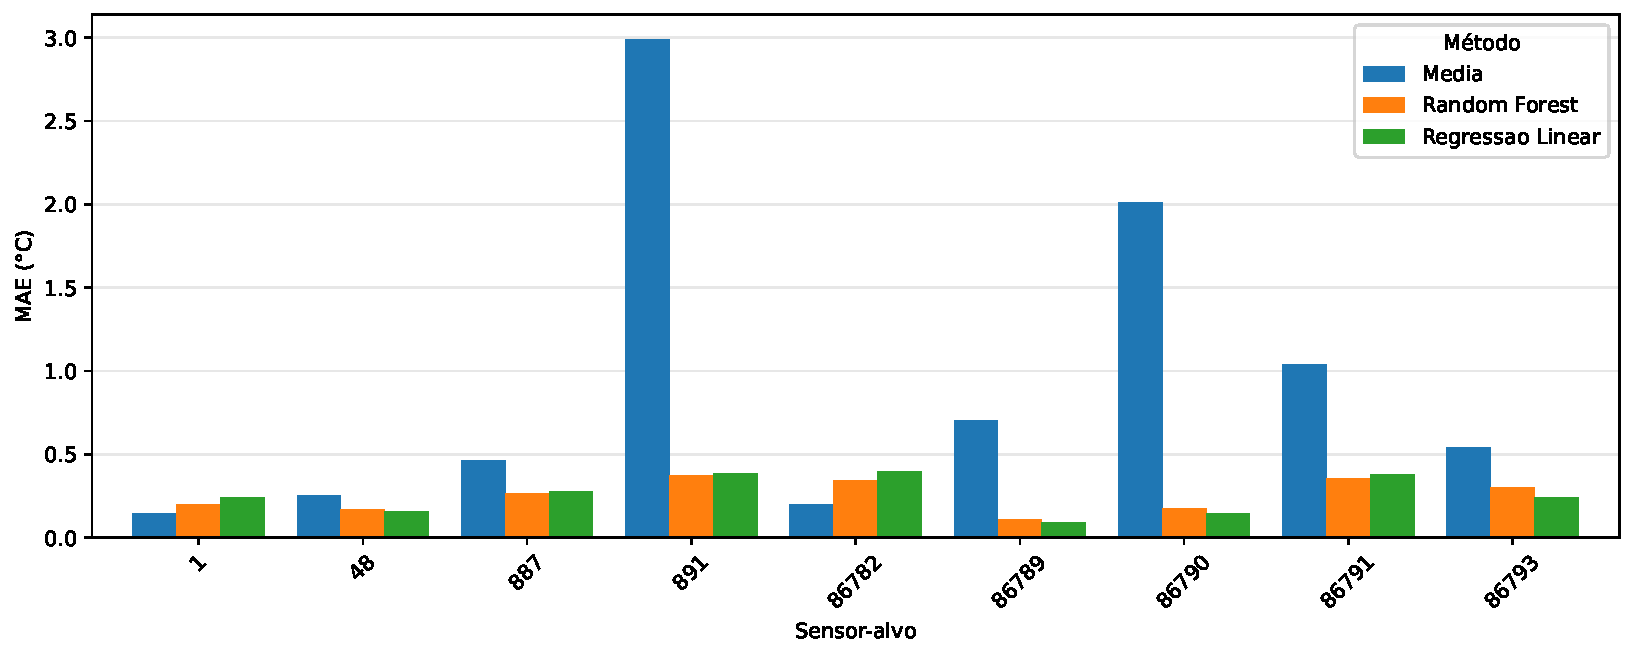
\includegraphics[width=\linewidth]{mae_por_sensor.pdf}
    \fautor
\end{figure}

O sensor 86789 apresentou o menor MAE supervisionado: 0,090~°C
com regressão linear, acompanhado de $R^2=0,985$. Já o sensor 891
apresentou MAE de 0,387~°C com regressão linear e 0,374~°C com
Random Forest, cujos $R^2$ foram, respectivamente, 0,442 e 0,448.
Assim, erros absolutos inferiores a meio grau nesse alvo coexistiram
com uma parcela relevante de variação não explicada pelos modelos.

Nos sensores 1 e 86782, a média aritmética obteve MAE de 0,145~°C
e 0,198~°C, respectivamente, abaixo dos dois modelos supervisionados.
Esse resultado evidencia a importância de manter uma referência
simples e avaliar cada alvo. O ajuste no treinamento não garante
menor erro no período posterior para todos os dispositivos.

A Figura~\ref{fig:reconstrucao_891} apresenta o sensor 891 como
exemplo das dificuldades de reconstrução, escolhido por seu maior
MAE entre os alvos na Random Forest. Os gráficos dos demais alvos
foram igualmente exportados. Nesse exemplo, a média aritmética
permanece acima da temperatura observada, enquanto as estimativas
supervisionadas acompanham melhor seu nível, mas ainda apresentam
resíduos positivos em parte do teste. A figura permite visualizar
esse comportamento, sem estabelecer sua causa física.

\begin{figure}[htbp]
    \centering
    \caption{Temperaturas observadas, estimativas e resíduos do sensor 891.}
    \label{fig:reconstrucao_891}
    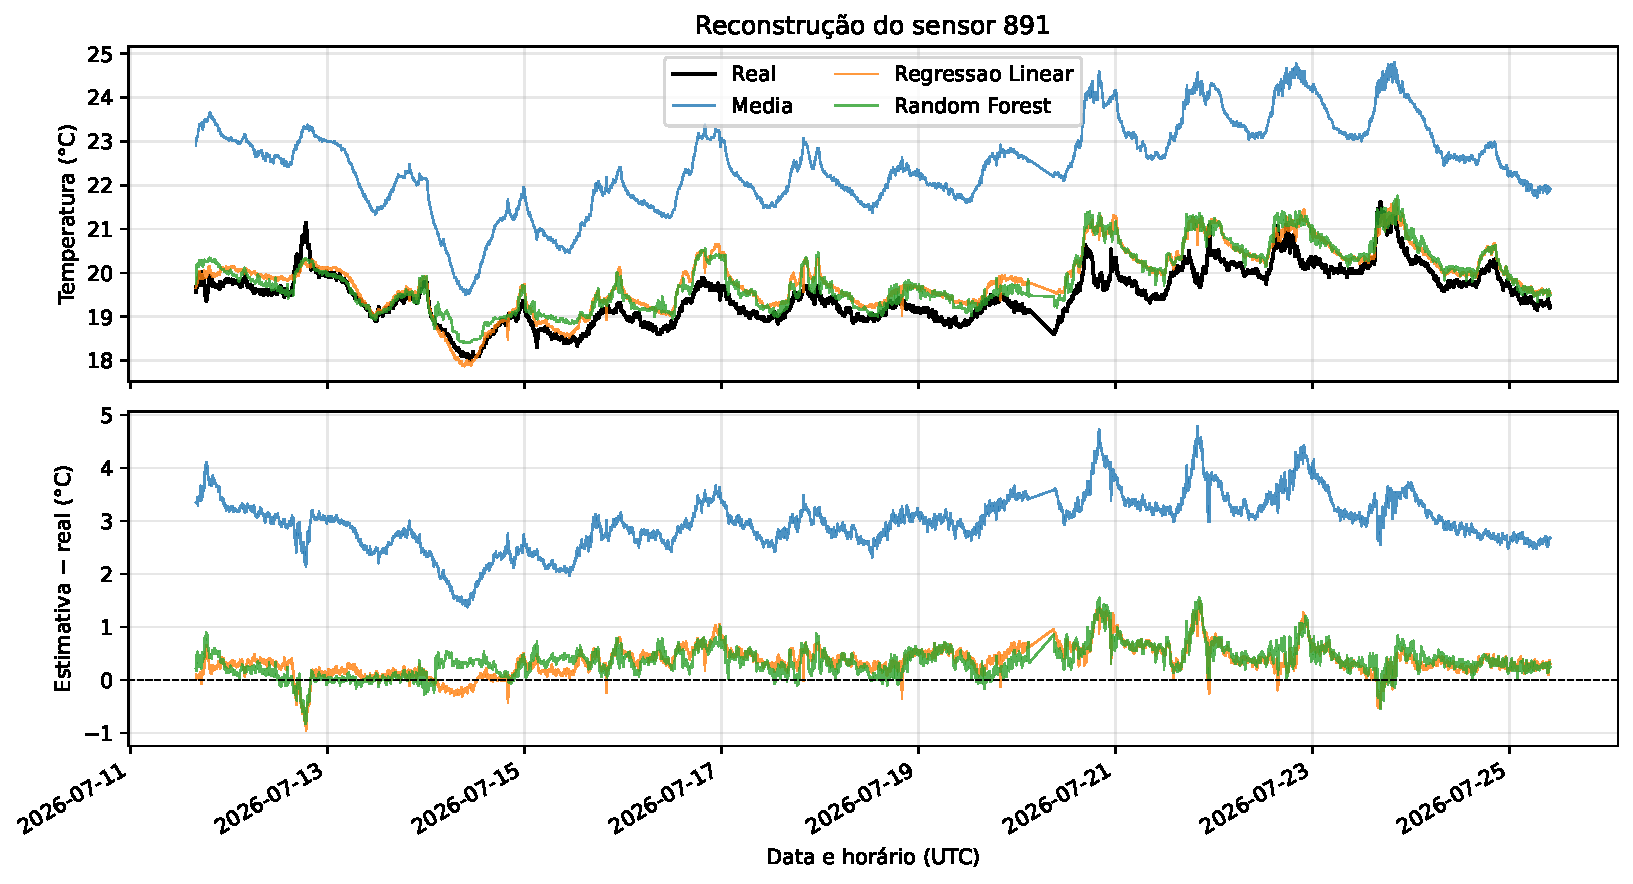
\includegraphics[width=\linewidth]{reconstrucao_sensor_891.pdf}
    \fautor
\end{figure}

\subsection{Influência da quantidade de entradas}
\label{subsec:resultados_quantidade}

A Tabela~\ref{tab:quantidade_sensores} apresenta os resultados da
regressão linear com seleção por correlação no treinamento.
O MAE médio diminuiu de 0,296~°C com uma entrada para 0,238~°C
com quatro. Com seis e oito entradas, os valores aumentaram para
0,257~°C, aproximadamente. A média dos RMSE também atingiu seu
menor valor entre as configurações avaliadas com quatro entradas,
igual a 0,302~°C.

\begin{table}[htbp]
    \centering
    \caption{Médias das métricas da regressão linear por quantidade de entradas.}
    \label{tab:quantidade_sensores}
    \begin{tabular}{rrrr}
\toprule
$k$ & MAE (°C) & RMSE (°C) & $R^2$ \\
\midrule
1 & 0,296 & 0,370 & 0,816 \\
2 & 0,255 & 0,322 & 0,855 \\
3 & 0,245 & 0,311 & 0,875 \\
4 & 0,238 & 0,302 & 0,880 \\
6 & 0,257 & 0,325 & 0,864 \\
8 & 0,257 & 0,325 & 0,850 \\
\bottomrule
\end{tabular}

    \fautor
\end{table}

A Figura~\ref{fig:quantidade_sensores} evidencia que o comportamento
varia conforme o alvo. Para o sensor 86782, por exemplo, o erro
cresce ao aumentar o número de entradas no ordenamento adotado,
enquanto outros sensores se beneficiam da inclusão de variáveis.
Portanto, o menor erro médio com quatro entradas não implica que
esse número seja preferível para todos os alvos.

\begin{figure}[htbp]
    \centering
    \caption{Erros por alvo e médias em função da quantidade de entradas.}
    \label{fig:quantidade_sensores}
    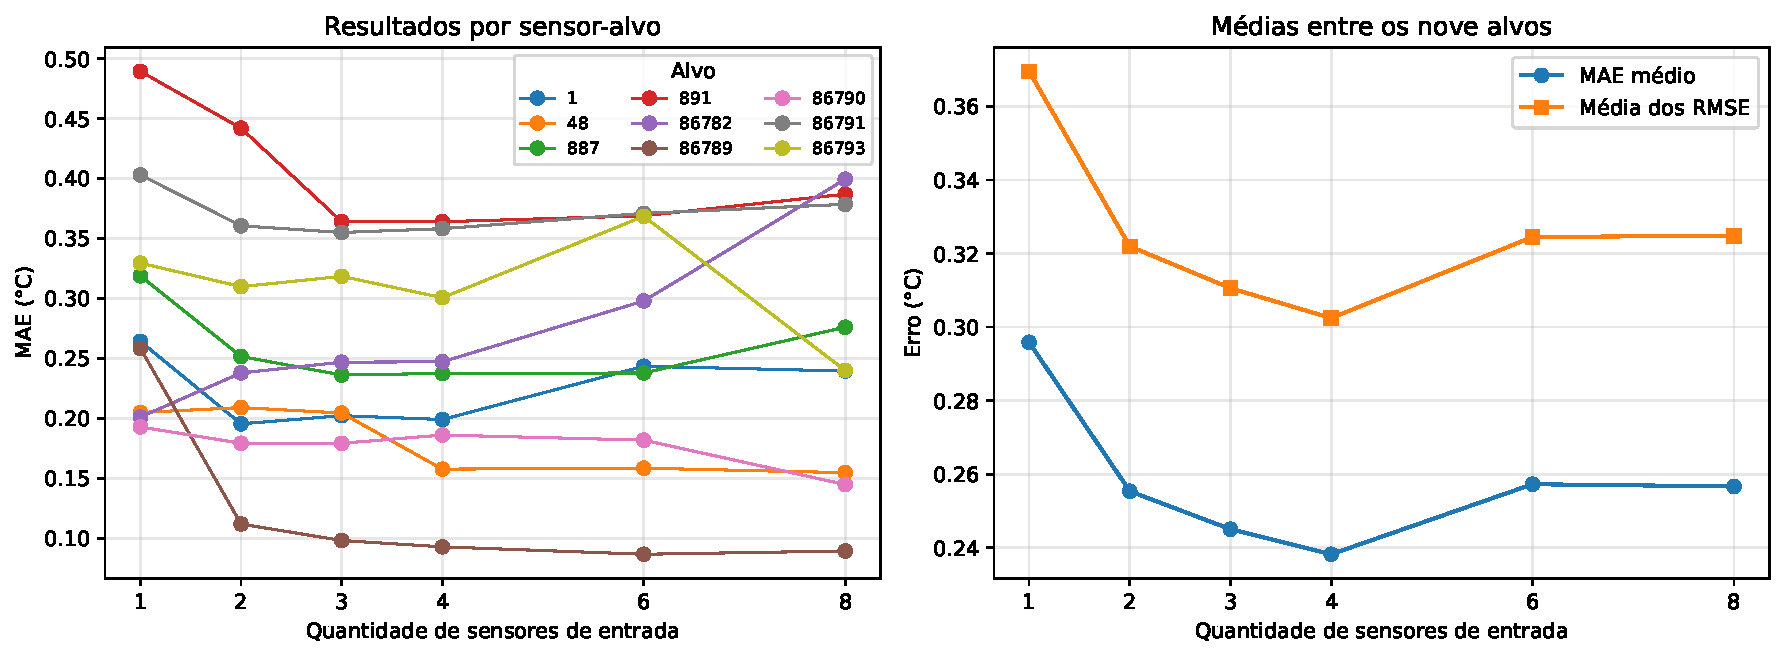
\includegraphics[width=\linewidth]{erro_quantidade_sensores.pdf}
    \fautor
\end{figure}

Esses resultados indicam que, neste período e com essa regra de
seleção, utilizar todos os sensores disponíveis não produziu o
menor erro médio. Entretanto, não demonstram que a seleção por
correlação supera outros critérios, pois não houve comparação
com subconjuntos aleatórios ou selecionados por distância nesse conjunto
de nove sensores. A comparação espacial complementar utiliza um recorte
comum de seis sensores e é apresentada na
Seção~\ref{subsec:resultados_espaciais}.
Também não estabelecem uma quantidade ótima geral: quatro foi
o menor erro observado entre os valores de $k$ examinados nesse
teste, sem uma avaliação independente posterior à escolha.

\subsection{Disponibilidade dos dados nas fontes consultadas}
\label{subsec:disponibilidade_fontes}

As extrações locais evidenciam diferenças no conjunto de dispositivos
consultados em cada fonte. O experimento principal contém nove sensores
do ambiente 1006 no QuestDB. A coleta pela API Smartlab contém 14
sensores com coordenadas: seis do ambiente 1006, seis do cluster e
dois cadastrados na reunião. Seis identificadores estão presentes
em ambas as extrações. Os sensores 1, 86782 e 86789 fazem parte da
extração principal do QuestDB, mas não da coleta local de 14 sensores
da Smartlab. Essa ausência decorre do inventário consultado e não
demonstra indisponibilidade desses dispositivos em toda a API.

Na consulta exploratória ao QuestDB preservada no notebook original,
a busca pelos seis identificadores do cluster retornou um conjunto
vazio, enquanto a API permitiu obter registros desses mesmos dispositivos.
Esse achado documenta o resultado das consultas realizadas, sem
estabelecer que as duas fontes tenham cobertura histórica equivalente
ou que o estado dos servidores permaneça o mesmo.

As respostas locais da API contêm timestamps sem indicação de fuso
e intervalos observados inferiores aos cinco minutos solicitados na
configuração exploratória. Assim, a contagem dessas linhas não pode
ser comparada diretamente à quantidade de janelas válidas do QuestDB.
A equiparação exige verificar a semântica temporal e a agregação antes
de combinar os dados. Por esse motivo, o mapa e a avaliação espacial
utilizam somente temperaturas do QuestDB, embora mostrem as posições
cadastradas dos demais dispositivos.

\subsection{Coordenadas e comparação da seleção espacial}
\label{subsec:resultados_espaciais}

A Tabela~\ref{tab:coordenadas} relaciona as posições confirmadas dos
seis sensores usados na análise complementar. As médias dessa tabela
utilizam somente as janelas completas comuns aos nove sensores do
experimento principal, diferentemente das estatísticas por sensor
da Tabela~\ref{tab:caracterizacao_sensores}.

\begin{table}[htbp]
    \centering
    \caption{Coordenadas relativas e médias nas 12.892 janelas comuns.}
    \label{tab:coordenadas}
    \begin{tabular}{rrrr}
\toprule
Sensor & X relativo & Y relativo & Média (°C) \\
\midrule
48 & 8,0 & 5,6 & 22,114 \\
887 & 0,0 & 0,0 & 22,618 \\
891 & 0,0 & 4,9 & 19,850 \\
86790 & 3,0 & 1,4 & 24,019 \\
86791 & 5,0 & 1,4 & 23,276 \\
86793 & 8,0 & 0,0 & 22,497 \\
\bottomrule
\end{tabular}

    \fautor
\end{table}

A Tabela~\ref{tab:selecao_espacial} e a Figura~\ref{fig:selecao_espacial}
apresentam a comparação entre seleção por correlação e por proximidade.
Para uma a quatro entradas, a correlação apresentou menor MAE médio
entre os seis alvos. Com uma entrada, os MAE médios foram 0,315~°C
para correlação e 0,390~°C para proximidade; com quatro, foram
0,276~°C e 0,295~°C, respectivamente. A média dos RMSE também foi
menor para a seleção por correlação nesses quatro valores de $k$.

\begin{table}[htbp]
    \centering
    \caption{Seleção por correlação e proximidade: médias entre seis alvos (°C).}
    \label{tab:selecao_espacial}
    \begin{tabular}{rrrrr}
\toprule
$k$ & MAE corr. & RMSE corr. & MAE prox. & RMSE prox. \\
\midrule
1 & 0,315 & 0,417 & 0,390 & 0,488 \\
2 & 0,298 & 0,379 & 0,374 & 0,458 \\
3 & 0,285 & 0,365 & 0,367 & 0,459 \\
4 & 0,276 & 0,353 & 0,295 & 0,374 \\
5 & 0,266 & 0,346 & 0,266 & 0,346 \\
\bottomrule
\end{tabular}

    \fonte{Autor desta monografia. Corr.: correlação; prox.: proximidade.}
\end{table}

\begin{figure}[htbp]
    \centering
    \caption{Desempenho da regressão linear com duas regras de seleção.}
    \label{fig:selecao_espacial}
    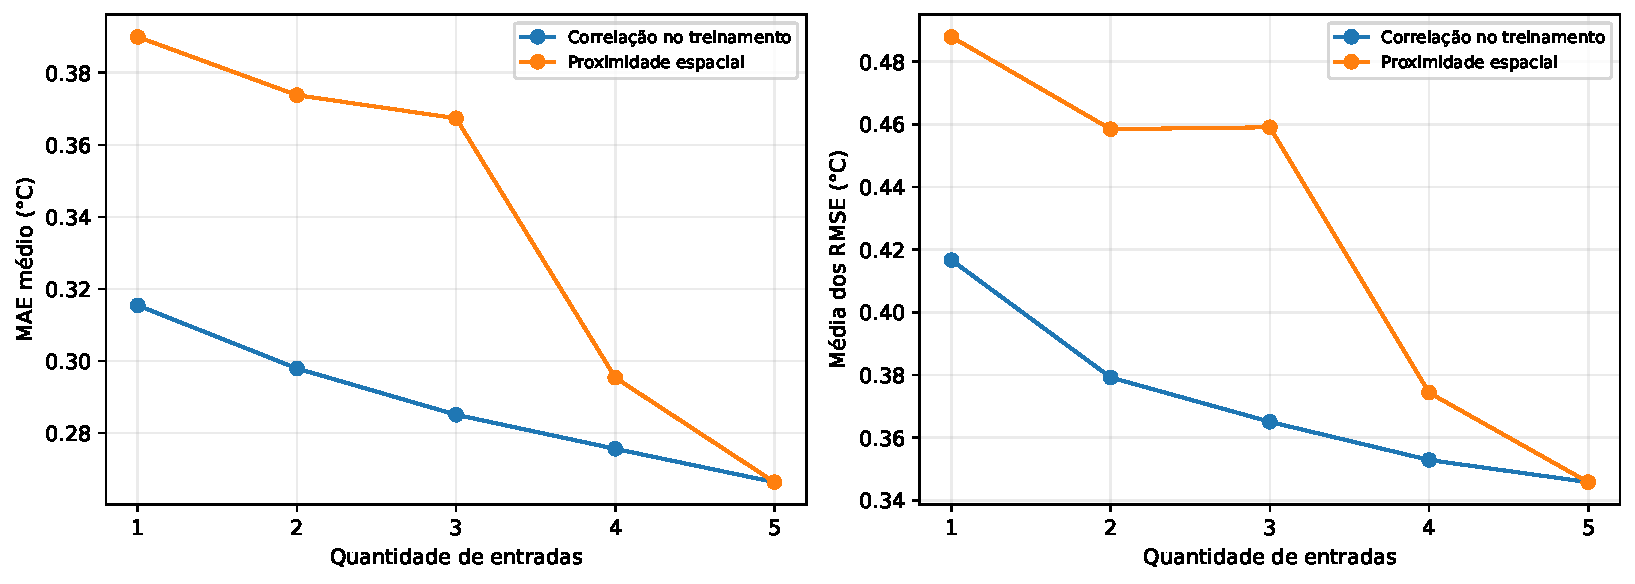
\includegraphics[width=\linewidth]{comparacao_selecao_espacial.pdf}
    \fautor
\end{figure}

Com cinco entradas, as duas regras utilizaram o mesmo conjunto de
sensores e produziram MAE médio de 0,266~°C e média dos RMSE de
0,346~°C. A concordância confirma a consistência dessa comparação.
Os resultados sugerem que a distância, isoladamente, não capturou
as relações úteis à regressão tão bem quanto a correlação histórica
nessa configuração. Não foi realizado teste de significância ou
validação em períodos adicionais para generalizar essa diferença.

A seleção espacial é uma análise com seis candidatos e seis alvos.
Seus erros médios não devem ser comparados diretamente aos da
Tabela~\ref{tab:quantidade_sensores}, que considera nove sensores.
Em particular, o menor erro com cinco entradas neste recorte não
contradiz o resultado com quatro entradas no conjunto anterior.
A divisória também não foi avaliada como variável explicativa ou
como efeito causal: ela é uma condição física documentada, e os
sensores do cluster foram excluídos dos candidatos de ambas as regras.

\subsection{Distribuição espacial das temperaturas médias}
\label{subsec:mapa_termico}

A Figura~\ref{fig:mapa_termico} apresenta os valores médios medidos
nos seis pontos e a interpolação ilustrativa entre eles. O sensor
891, localizado abaixo da divisória, apresentou média de 19,850~°C,
enquanto o sensor 86790 apresentou 24,019~°C. A figura permite
situar espacialmente essa diferença, sem atribuí-la à divisória,
aos equipamentos ou à climatização.

\begin{figure}[htbp]
    \centering
    \caption{Temperaturas médias observadas e interpolação IDW ilustrativa.}
    \label{fig:mapa_termico}
    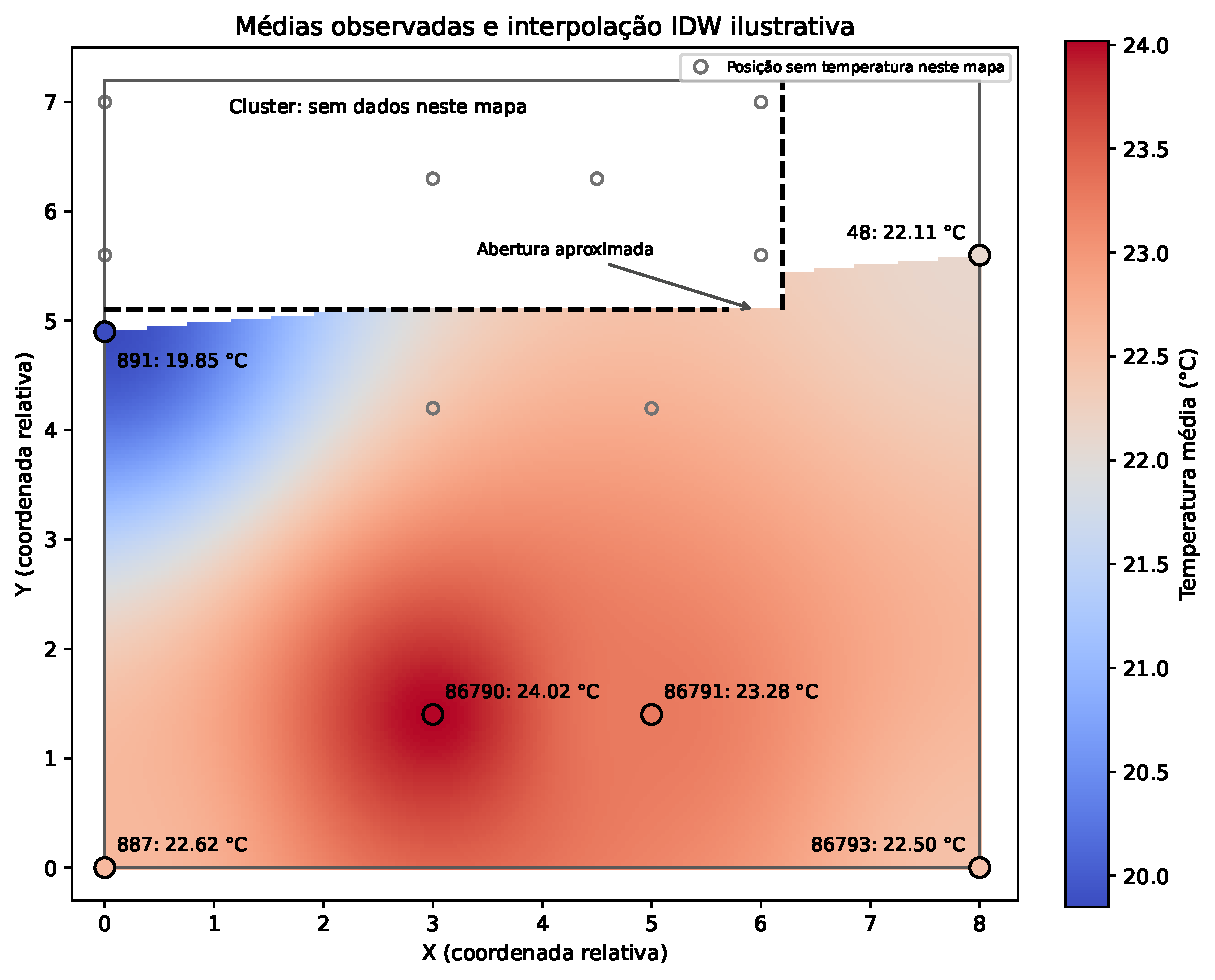
\includegraphics[width=0.95\linewidth]{mapa_termico_1006_painel.pdf}
    \fonte{Autor desta monografia. Geometria aproximada a partir da planta;
    pontos coloridos: médias observadas; fundo: interpolação das médias.
    Regiões sem preenchimento não foram estimadas.}
\end{figure}

A área do cluster permanece sem preenchimento, evitando apresentar
uma continuidade interpolada através da divisória. As paredes
tracejadas e a abertura aproximada indicam a limitação geométrica
da representação. A IDW suaviza as médias entre os pontos observados,
mas não fornece evidência de que as temperaturas nas posições sem
sensores correspondam aos valores coloridos. O mapa complementa a
caracterização dos dados; a validação quantitativa continua restrita
aos sensores físicos usados como alvos.

\subsection{Caracterização da umidade e efeito do enriquecimento}
\label{subsec:resultados_umidade}

A Tabela~\ref{tab:umidade_sensores} apresenta a disponibilidade da
umidade e as estatísticas das médias de cinco minutos, antes de
restringir as amostras à comparação pareada. A cobertura variou de
97,52\% a 97,85\% da grade. As umidades médias variaram de 53,98\%
no sensor 86790 a 59,80\% no sensor 891. O desvio é expresso em
pontos percentuais (p.p.), para distinguir a variação da UR de uma
variação percentual relativa à média.

\begin{table}[htbp]
    \centering
    \caption{Disponibilidade e estatísticas da umidade relativa agregada.}
    \label{tab:umidade_sensores}
    \begin{tabular}{rrrrr}
\toprule
Sensor & Janelas & Cobertura (\%) & Média (\%) & Desvio (p.p.) \\
\midrule
1 & 12944 & 97,71 & 56,65 & 8,47 \\
48 & 12919 & 97,52 & 54,52 & 8,06 \\
887 & 12931 & 97,61 & 57,66 & 7,48 \\
891 & 12954 & 97,78 & 59,80 & 7,09 \\
86782 & 12963 & 97,85 & 56,57 & 8,67 \\
86789 & 12938 & 97,66 & 57,14 & 8,25 \\
86790 & 12925 & 97,56 & 53,98 & 7,25 \\
86791 & 12941 & 97,68 & 56,75 & 7,25 \\
86793 & 12960 & 97,83 & 59,16 & 8,19 \\
\bottomrule
\end{tabular}

    \fautor
\end{table}

A Figura~\ref{fig:caracterizacao_umidade} mostra a evolução das
médias horárias, utilizadas apenas para legibilidade, e a proporção
de janelas válidas de cinco minutos. As correlações de Pearson
entre temperatura e umidade do mesmo dispositivo, calculadas no
treinamento, foram negativas nos nove sensores, entre $-0{,}446$
e $-0{,}108$. Esse diagnóstico não demonstra que a umidade forneça
informação preditiva adicional; essa possibilidade foi examinada
na comparação com entradas enriquecidas.

\begin{figure}[htbp]
    \centering
    \caption{Séries de umidade e disponibilidade das janelas no período.}
    \label{fig:caracterizacao_umidade}
    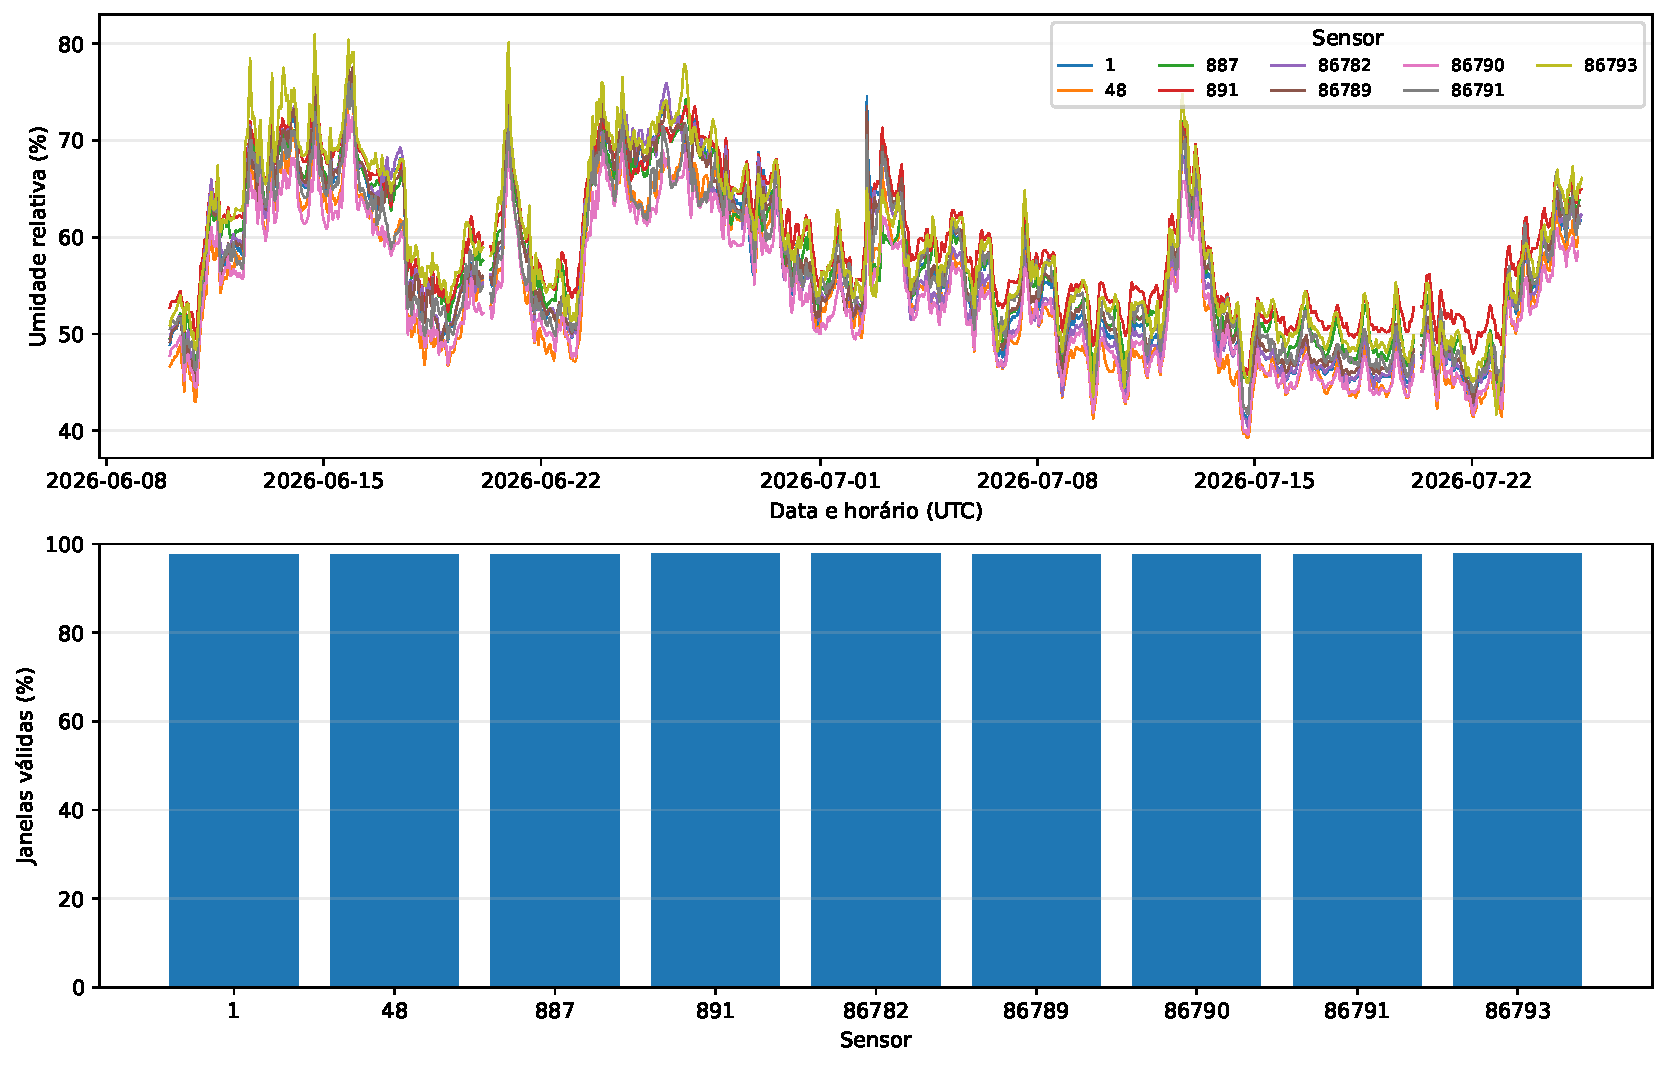
\includegraphics[width=0.95\linewidth]{caracterizacao_umidade.pdf}
    \fautor
\end{figure}

Na Tabela~\ref{tab:enriquecimento_umidade}, o acréscimo de umidade
reduziu o MAE médio da regressão linear de 0,25668~°C para
0,25343~°C, uma diferença de aproximadamente 0,00325~°C.
A média dos RMSE passou de 0,32488~°C para 0,32250~°C.
O ganho agregado foi pequeno e não foi submetido a teste de
significância ou confirmado em períodos independentes.

\begin{table}[htbp]
    \centering
    \caption{Regressão linear com e sem umidade, nas mesmas amostras por alvo.}
    \label{tab:enriquecimento_umidade}
    \begin{tabular}{lrrr}
\toprule
Entradas & MAE (°C) & RMSE (°C) & $R^2$ \\
\midrule
Temperaturas & 0,25668 & 0,32488 & 0,850 \\
Temperaturas e umidades & 0,25343 & 0,32250 & 0,857 \\
\bottomrule
\end{tabular}

    \fautor
\end{table}

A Tabela~\ref{tab:umidade_por_alvo} e a Figura~\ref{fig:efeito_umidade}
mostram que o enriquecimento reduziu o MAE em cinco alvos e aumentou
em quatro. O sensor 891 apresentou redução de 0,38690~°C para
0,33541~°C; já o sensor 86782 passou de 0,39943~°C para
0,45071~°C. Assim, acrescentar uma grandeza ambiental não assegurou
melhora uniforme. A avaliação não permite atribuir o resultado a
uma causa específica, como posição, climatização ou mecanismo físico
entre temperatura e umidade.

\begin{table}[htbp]
    \centering
    \caption{Efeito da umidade no MAE por alvo; diferença negativa indica redução.}
    \label{tab:umidade_por_alvo}
    \begin{tabular}{rrrr}
\toprule
Sensor & Somente T (°C) & T e UR (°C) & $\Delta$ MAE (°C) \\
\midrule
1 & 0,240 & 0,228 & -0,011 \\
48 & 0,155 & 0,169 & 0,014 \\
887 & 0,276 & 0,241 & -0,035 \\
891 & 0,387 & 0,335 & -0,051 \\
86782 & 0,399 & 0,451 & 0,051 \\
86789 & 0,090 & 0,119 & 0,029 \\
86790 & 0,145 & 0,148 & 0,003 \\
86791 & 0,379 & 0,361 & -0,018 \\
86793 & 0,240 & 0,229 & -0,011 \\
\bottomrule
\end{tabular}

    \fautor
\end{table}

\begin{figure}[htbp]
    \centering
    \caption{MAE da regressão linear com e sem umidade dos sensores de entrada.}
    \label{fig:efeito_umidade}
    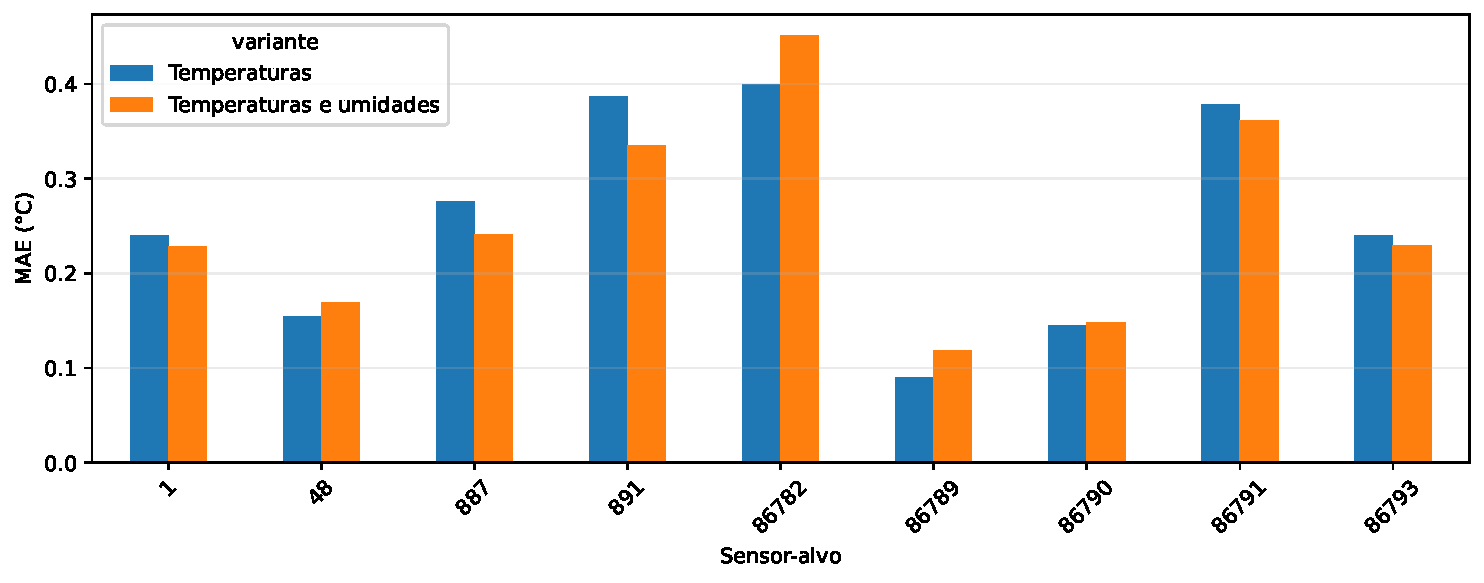
\includegraphics[width=\linewidth]{efeito_umidade.pdf}
    \fautor
\end{figure}

As duas variantes compartilham amostras em cada alvo, mas há duas
linhas de teste a menos para oito alvos em relação ao experimento
principal. Por isso, a referência dessa comparação é a regressão
reajustada com somente temperaturas, e não uma comparação direta
com a Random Forest ou com as médias da
Tabela~\ref{tab:comparacao_modelos}. A análise mantém temperatura
como resposta; a reconstrução da própria umidade não foi avaliada.

\subsection{Disponibilidade e interpretação dos registros de energia}
\label{subsec:resultados_energia}

A consulta à tabela de energia retornou registros apenas do sensor 23
no período selecionado: 8.193 linhas, entre 10/06/2026 às
01h43min35s e 11/06/2026 às 22h31min36s, em UTC. O sensor 2,
identificado na exploração histórica, não retornou dados nesse
recorte. A agregação produziu 539 janelas válidas, correspondentes
a 4,07\% das 13.248 previstas. Portanto, essa fonte não oferece
cobertura comparável à de temperatura e umidade ao longo das seis
semanas analisadas.

Os valores brutos do campo variaram de 0 a 9,13. As médias de cinco
minutos variaram de 0 a 6,865, na escala registrada no banco.
Como a unidade e a transformação do firmware não foram confirmadas,
esses valores não são interpretados como kWh, W ou A. A
Figura~\ref{fig:energia_exploratoria} apresenta apenas a sobreposição
dos registros disponíveis e das temperaturas no mesmo trecho.

\begin{figure}[htbp]
    \centering
    \caption{Campo de energia e temperaturas no curto intervalo disponível.}
    \label{fig:energia_exploratoria}
    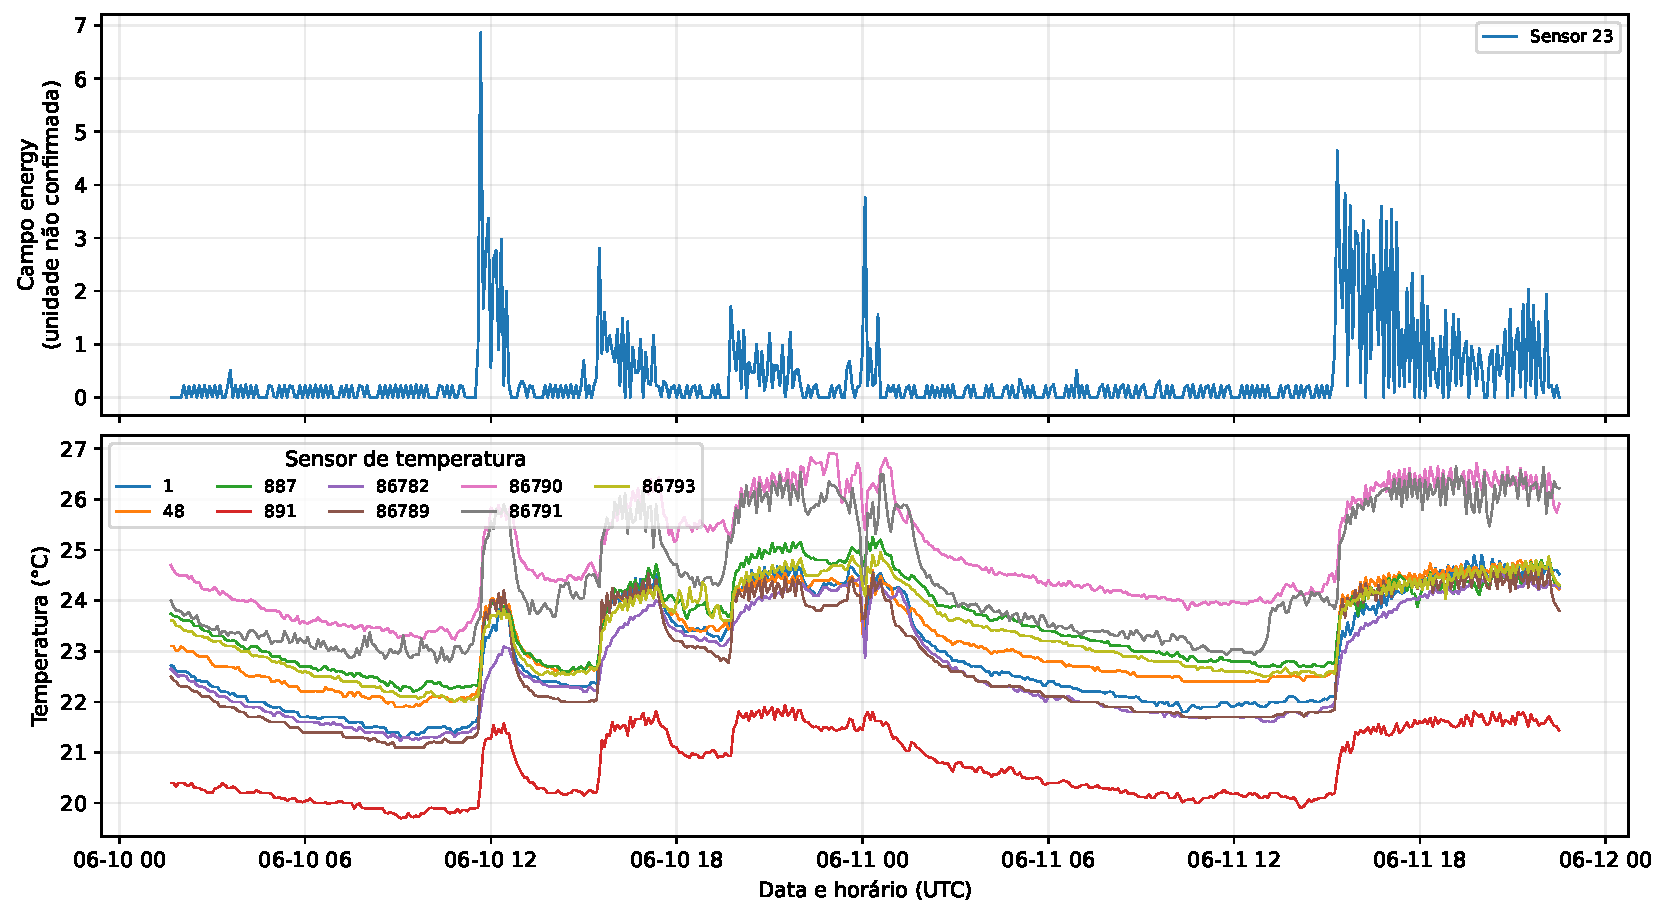
\includegraphics[width=\linewidth]{energia_temperatura_exploratoria.pdf}
    \fautor
\end{figure}

A série apresenta variações na escala registrada, mas sua sobreposição
às temperaturas não identifica, por si só, estados do ar-condicionado
ou efeitos causais. A curta disponibilidade e a unidade pendente de
confirmação limitaram o uso desses dados à auditoria e à visualização,
sem incluí-los como entradas dos modelos ou calcular consumo energético.

\subsection{Síntese e alcance dos resultados}
\label{subsec:sintese_resultados}

No conjunto estudado, foi possível reconstruir as médias de
temperatura dos nove sensores com MAE médio entre alvos próximo
de 0,25~°C usando métodos supervisionados. A adequação desse erro
a uma aplicação específica dependeria de requisitos que não foram
definidos neste experimento. A regressão linear e a Random Forest
apresentaram desempenho agregado próximo, com vantagens distintas
conforme a métrica e o alvo. A análise de quantidade mostrou que
mais entradas não asseguraram menor erro no período de teste.

A umidade acrescentou um ganho médio pequeno, com efeitos distintos
por alvo, enquanto os registros de energia tiveram disponibilidade
insuficiente para uma avaliação no período completo.
A evidência se restringe à reconstrução de janelas completas em
um ambiente e uma divisão temporal. Não foi avaliada a operação
sob indisponibilidade simultânea das entradas, nem a estabilidade
em outras estações, ambientes ou configurações físicas. Além disso,
a referência é a medição do sensor físico: concordância com esse
registro não demonstra exatidão em relação a um instrumento calibrado,
nem valida índices de conforto térmico ou um campo térmico contínuo.



\section{Dificuldades e Limitações}
\label{sec:dificuldades_limitacoes}

A sincronização exigiu agregar medições cujos instantes de aquisição
não coincidem. A exclusão de 356 janelas incompletas permitiu comparar
os métodos nas mesmas amostras, mas restringe a avaliação a instantes
com todas as entradas disponíveis. Portanto, os resultados não medem
o desempenho durante falhas simultâneas dos sensores de entrada.
As médias de cinco minutos também foram calculadas com quantidades
variáveis de medições, sem impor um limite mínimo uniforme.

A avaliação utiliza um único ambiente, um período e uma divisão
cronológica. A dependência temporal entre observações e a ausência
de repetições em outros períodos limitam as conclusões de generalização.
O teste foi examinado em diferentes configurações exploratórias;
por isso, o menor erro observado não deve ser interpretado como
avaliação independente de uma configuração escolhida após essa inspeção.
Não foram estimados intervalos de confiança nem significância
estatística das diferenças entre métodos.

As coordenadas estão disponíveis para seis dos nove sensores, e as
paredes foram aproximadas a partir da planta. A distância euclidiana
não modela obstáculos, circulação de ar ou trocas de calor pela abertura.
O mapa interpola médias observadas e não valida um campo térmico contínuo.
A separação dos registros do QuestDB e da API evita combinar convenções
temporais ainda não equiparadas, mas deixa as medições do cluster fora
da avaliação consolidada.

A extensão com umidade foi avaliada no mesmo período já examinado
nos experimentos anteriores, sem constituir teste independente de
novas hipóteses em dados inéditos. Para energia, a curta disponibilidade
e a unidade não confirmada impedem interpretar os valores como consumo.

Por fim, a referência experimental é o registro de cada sensor, sem
comparação com instrumento calibrado. Assim, erro reduzido de reconstrução
não demonstra exatidão metrológica nem atendimento a critérios de
conforto térmico. A contribuição está na avaliação dos métodos nas
condições documentadas, com dados, parâmetros e previsões rastreáveis.

\section{Considerações Finais}
\label{sec:desenvolvimento_finais}

A avaliação mostrou erros agregados próximos entre regressão linear
e Random Forest, com vantagens distintas conforme o alvo e a métrica.
A quantidade de entradas e a regra de seleção influenciaram os erros;
a análise espacial permitiu situar as diferenças de temperatura e
comparar proximidade com correlação em condições comuns. O capítulo
seguinte sintetiza essas evidências e suas possibilidades de continuidade.

\chapter{Conclusão}
\label{sec:conclusao}

Este trabalho investigou a reconstrução virtual de temperaturas
a partir de medições de sensores IoT instalados no ambiente 1006
do LASDPC. O objetivo proposto foi atendido por meio da preparação,
sincronização e enriquecimento de dados históricos de nove sensores
físicos, cujas medições foram agregadas em intervalos de cinco
minutos. A avaliação permitiu comparar métodos de reconstrução
e investigar a influência da quantidade e da seleção de sensores
de referência, bem como a contribuição de informações ambientais
complementares. A principal contribuição consiste na avaliação
experimental dessas estratégias em uma infraestrutura real
preexistente, com procedimentos e resultados documentados
para reprodução.

Na comparação principal, os métodos supervisionados apresentaram
erros médios inferiores aos da média aritmética. A regressão
linear obteve MAE médio entre sensores-alvo de 0,257~°C,
enquanto a Random Forest alcançou 0,254~°C, em comparação
a 0,927~°C da referência. A Random Forest apresentou o menor
MAE médio, enquanto a regressão linear obteve a menor média
dos RMSE. Entretanto, as diferenças agregadas entre os modelos
supervisionados foram pequenas e o desempenho variou conforme
o sensor-alvo. A média aritmética, por exemplo, apresentou
menor MAE nos sensores 1 e 86782, evidenciando que nenhuma
das abordagens foi superior em todos os casos.

Diante desses resultados, a regressão linear se apresenta
como uma alternativa inicial competitiva para a reconstrução
de temperaturas no cenário estudado, considerando sua
simplicidade estrutural e seu desempenho próximo ao da
Random Forest. Essa interpretação não estabelece superioridade
estatística nem exclui a utilização de outros métodos,
especialmente em sensores para os quais foram observadas
vantagens individuais.

A investigação da quantidade de entradas mostrou que
utilizar todos os sensores disponíveis não necessariamente
produz estimativas mais precisas. Na regressão linear com
seleção por correlação calculada exclusivamente no treinamento,
quatro sensores de referência apresentaram o menor MAE médio
entre as configurações avaliadas, de 0,238~°C. Esse resultado
sugere que subconjuntos de sensores podem oferecer informações
suficientes para reconstruções competitivas. Entretanto,
o desempenho depende do sensor-alvo e da regra de seleção
empregada, não sendo possível estabelecer uma quantidade
universalmente ótima com base nos experimentos realizados.

Na análise espacial complementar, realizada com seis sensores
de posições conhecidas, a seleção por correlação histórica
apresentou menor MAE médio que a seleção por proximidade
física para uma a quatro entradas. Esse comportamento indica
que a distância euclidiana, isoladamente, não foi o critério
mais favorável nas configurações avaliadas. A representação
espacial das temperaturas médias também permitiu visualizar
diferenças entre os dispositivos, utilizando interpolação
IDW exclusivamente para fins ilustrativos, sem validar
um campo térmico contínuo.

O enriquecimento das entradas com umidade relativa produziu
uma redução pequena no MAE médio da regressão linear, com
melhorias em cinco sensores-alvo e aumento do erro nos
outros quatro. Dessa forma, não foi observada uma vantagem
uniforme da inclusão dessa grandeza nas condições avaliadas.
Os registros de energia, por sua vez, apresentaram baixa
disponibilidade temporal, cobrindo apenas 4,07\% da grade
considerada, e não tiveram sua unidade física confirmada.
Por esse motivo, sua utilização permaneceu restrita a uma
análise exploratória.

As conclusões obtidas estão limitadas a um único ambiente,
um período de observação e uma divisão cronológica de
treinamento e teste, considerando apenas janelas com
temperaturas disponíveis para todos os sensores do conjunto
principal. Não foram avaliados cenários de indisponibilidade
simultânea das entradas ou a estabilidade dos modelos em
outras condições ambientais. Além disso, as medições dos
próprios sensores foram utilizadas como referência,
sem comparação com instrumentos calibrados. Portanto,
os erros observados não demonstram exatidão metrológica
nem validam diretamente a reconstrução de temperaturas
em posições não instrumentadas ou a avaliação de conforto
térmico.

Como continuidade, recomenda-se avaliar os métodos em
outros períodos e ambientes, investigar estratégias de
reconstrução diante de falhas dos sensores de referência
e validar estimativas em posições não instrumentadas.
A integração de novas fontes de dados, após a verificação
de suas convenções temporais e unidades físicas, também
poderá ampliar as possibilidades de análise. Por fim,
a utilização das temperaturas reconstruídas em estudos
de conforto térmico dependerá da definição de um protocolo
específico e da obtenção das demais variáveis ambientais
e pessoais necessárias.

Em síntese, os resultados demonstram que dados históricos
de uma infraestrutura IoT existente podem ser utilizados
para reconstruir temperaturas de sensores físicos com
erros relativamente baixos nas condições experimentais
avaliadas. A comparação entre métodos e configurações
evidencia a importância de considerar as características
de cada sensor-alvo e de selecionar adequadamente as
informações utilizadas na reconstrução, oferecendo uma
base experimental para futuras aplicações de sensoriamento
virtual no LASDPC.

\postextual
\phantomsection
\addcontentsline{toc}{chapter}{REFERÊNCIAS}
\bibliography{references}

\end{document}
